% \usepackage{xcolor}
\usepackage[table,usenames,dvipsnames]{xcolor}

\usepackage{amsmath,amssymb,amsfonts}
\usepackage{graphicx}

\usepackage{nameref}

% For abbreviations, we use "acro" package, and mfirstuc to help capitalize long
% versions normally
\usepackage{mfirstuc}
\MFUhyphentrue % tell mfirstuc to capitalize hyphenated words

% Acronyms
\usepackage{acro}
% For one-offs,
% \DeclareAcronym{acronym}{short=short-version,long=long-version}

\newcommand{\newacr}[2]{\DeclareAcronym{#1}{short=\uppercase{#1},long=#2}}
\newcommand{\newacrs}[3]{\DeclareAcronym{#1}{short=#2,long=#3}}

% Alphabetically sorted list of acronyms
\newacr{aop}{Aspect-Oriented Programming}
\newacr{api}{Application Programming Interface}
\newacr{ast}{Abstract Syntax Tree}
\newacr{cms}{Content Management System}
\newacr{cpu}{Central Processing Unit}
\newacr{csv}{Comma-Separated Values}
\newacr{dsl}{Domain-Specific Language}
\newacr{ffi}{Foreign Function Interface}
\newacr{gui}{Graphical User Interface}
\newacr{html}{HyperText Markup Language}
\newacr{href}{Hypertext REFerence}
\newacr{ide}{Integrated Development Environment}
\newacr{json}{JavaScript Object Notation}
\newacr{jvm}{Java Virtual Machine}
\newacr{mop}{MetaObject Protocol}
\newacr{nasa}{National Aeronautics and Space Administration}
\newacr{pdf}{Portable Document Format}
\newacr{sst}{Skeleton Syntax Tree}
\newacr{wysiwyg}{What You See Is What You Get}

% Case Studies 
%   (note: I'm grouping these together and forcing "newacrs" usage, even when
%    seemingly unneeded because, otherwise, they won't group together at the 
%    bottom of the complete "acronyms" list.)
\newacrs{glassbr}{GlassBR}{Glass Breaking}
\newacrs{projectile}{Projectile}{Projectile}
\newacrs{sglpend}{SglPend}{Single Pendulum}
\newacrs{dblpend}{DblPend}{Double Pendulum}
\newacrs{gamephysics}{GamePhysics}{Game Physics}
\newacrs{hghc}{HGHC}{Heat Transfer Coefficients between Fuel and Cladding in Fuel Rods}
\newacrs{pdcontroller}{PDController}{Proportional Derivative Controller}
\newacrs{swhs}{SWHS}{Solar Water Heating System}
\newacrs{nopcm}{SWHSNoPCM}{Solar Water Heating System Without PCM}
\newacrs{ssp}{SSP}{Slope Stability analysis Program}


%------------------------------------------------------------------------------
%- Extra commands for more functionality -- in particular, capitalizing the
%- long form of acronyms.
%------------------------------------------------------------------------------

% Defining \ACL - to capitalize all words in an acronym
% Credits to: https://tex.stackexchange.com/a/257896
\NewDocumentCommand\ACF{sm}{%
  \begingroup
  \acsetup{uppercase/cmd=\ecapitalisewords}%
  \IfBooleanTF{#1}{\Acf*{#2}}{\Acf{#2}}%
  \endgroup
}

\NewDocumentCommand\ACFP{sm}{%
  \begingroup
  \acsetup{uppercase/cmd=\ecapitalisewords}%
  \IfBooleanTF{#1}{\Acfp*{#2}}{\Acfp{#2}}%
  \endgroup
}

\NewDocumentCommand\ACL{sm}{%
  \begingroup
  \acsetup{uppercase/cmd=\ecapitalisewords}%
  \IfBooleanTF{#1}{\Acl*{#2}}{\Acl{#2}}%
  \endgroup
}

\NewDocumentCommand\ACLP{sm}{%
  \begingroup
  \acsetup{uppercase/cmd=\ecapitalisewords}%
  \IfBooleanTF{#1}{\Aclp*{#2}}{\Aclp{#2}}%
  \endgroup
}


% General Assets
%------------------------------------------------------------------------------
% Code
%------------------------------------------------------------------------------

% Command based on: https://tex.stackexchange.com/questions/266811/define-a-new-command-with-parameters-inside-newcommand
\newcommand{\codeName}[1]{\expandafter\newcommand\csname #1\endcsname{\inlineHs{#1}}}

% Used for showing what the blue-highlighted text is, in the reading notes section
\codeName{ExampleText}

% Defines commands to be used in poster and thesis

\newcommand{\swebokScalDef}{This seems to define ``usability
    testing'' with elements of functional and recovery testing}
\newcommand{\swebokElasRef}{only cites a single source
    \textbf{that doesn't contain the words ``elasticity'' or ``elastic''}!}

% for assets/code/example.tex...
\newcommand{\exampleCode}{\begin{codeSnippet}{haskell}{``MultiDefinitions'' (MultiDefn) Definition}{exampleCode}{https://github.com/JacquesCarette/Drasil/blob/051b9881a6417e51e818c6673c5eab0f48bd5af2/code/drasil-theory/lib/Theory/Drasil/MultiDefn.hs\#L45-L56}
-- | 'MultiDefn's are QDefinition factories, used for showing one or more ways
--   we can define a QDefinition.
data MultiDefn e = MultiDefn{
  -- | UID
  _rUid :: UID,
  -- | Underlying quantity it defines.
  _qd :: QuantityDict,
  -- | Explanation of the different ways we can define a quantity.
  _rDesc :: Sentence,
  -- | All possible ways we can define the related quantity.
  _rvs :: NE.NonEmpty (DefiningExpr e)
}
\end{codeSnippet}
}
\newcommand{\refExampleCode}{\Cref{lst:exampleCode}}

% for assets/code/examplePseudocode.tex...
\newcommand{\examplePseudocode}{\begin{pseudocode}{haskell}{Broken QuantityDict Chunk Retriever}{examplePseudocode}
retrieveQD :: UID -> ChunkDB -> Maybe QuantityDict
retrieveQD u cdb = do
    (Chunk expectedQd) <- lookup u cdb
    pure expectedQd
\end{pseudocode}
}
\newcommand{\refExamplePseudocode}{\Cref{lst:examplePseudocode}}

% for assets/code/mainInvalidInputTest.tex...
\newcommand{\mainInvalidInputTest}{\begin{codeSnippet}{python}{Tests for main with an invalid input file}{mainInvalidInputTest}{https://github.com/samm82/Drasil/blob/sysTests/code/stable/projectile/projectile_c_p_nol_b_u_v_d/src/python/test/Control_test.py\#L29-L53}
  # from https://stackoverflow.com/questions/54071312/how-to-pass-command-line-argument-from-pytest-to-code
  ## \brief Tests main with invalid input file
  # \par Types of Testing:
  # Dynamic Black-Box (Behavioural) Testing
  # Boundary Conditions
  # Default, Empty, Blank, Null, Zero, and None
  # Invalid, Wrong, Incorrect, and Garbage Data
  # Logic Flow Testing
  @mark.parametrize("filename", invalid_value_input_files)
  @mark.xfail
  def test_main_invalid(monkeypatch, filename):
      # from https://stackoverflow.com/questions/10840533/most-pythonic-way-to-delete-a-file-which-may-not-exist
      try:
          remove(output_filename)
      except OSError as e: # this would be "except OSError, e:" before Python 2.6
          if e.errno != ENOENT: # no such file or directory
              raise # re-raise exception if a different error occurred


      assert not path.exists(output_filename)


      with monkeypatch.context() as m:
          m.setattr(sys, 'argv', ['Control.py', str(Path("test/test_input") / f"{filename}.txt")])
          Control.main()
      
      assert not path.exists(output_filename)
\end{codeSnippet}
}
\newcommand{\refMainInvalidInputTest}{\Cref{lst:mainInvalidInputTest}}

% for assets/code/projManualViolationReq.tex...
\newcommand{\projManualViolationReq}{\begin{codeSnippet}{haskell}{\acs{projectile}'s manually created requirement for constraint violation behaviour}{projManualViolationReq}{https://github.com/JacquesCarette/Drasil/blob/afb6fb752b8364d2807ced7fc0c1dd6c6aba52b2/code/drasil-example/projectile/lib/Drasil/Projectile/Requirements.hs\#L31-L34}
verifyParamsDesc = foldlSent [S "Check the entered", plural inValue,
    S "to ensure that they do not exceed the" +:+. namedRef (datCon [] []) (plural datumConstraint),
    S "If any of the", plural inValue, S "are out of bounds" `sC`
    S "an", phrase errMsg, S "is displayed" `S.andThe` plural calculation, S "stop"]
\end{codeSnippet}
}
\newcommand{\refProjManualViolationReq}{\Cref{lst:projManualViolationReq}}

% for assets/code/projViolationChoice.tex...
\newcommand{\projViolationChoice}{\begin{codeSnippet}{haskell}{\acs{projectile}'s choice for constraint violation behaviour in code}{projViolationChoice}{https://github.com/JacquesCarette/Drasil/blob/afb6fb752b8364d2807ced7fc0c1dd6c6aba52b2/code/drasil-example/projectile/lib/Drasil/Projectile/Choices.hs\#L120}
    srsConstraints = makeConstraints Warning Warning,
\end{codeSnippet}
}
\newcommand{\refProjViolationChoice}{\Cref{lst:projViolationChoice}}

%------------------------------------------------------------------------------
% Graphs
%------------------------------------------------------------------------------

% Organization of files

\newcommand{\parChdGraphs}{
    % Only top or bottom to comply with IEEE guidelines
    \begin{figure}[bt!]
        \centering
        \begin{subfigure}[b]{\linewidth}
            \centering
            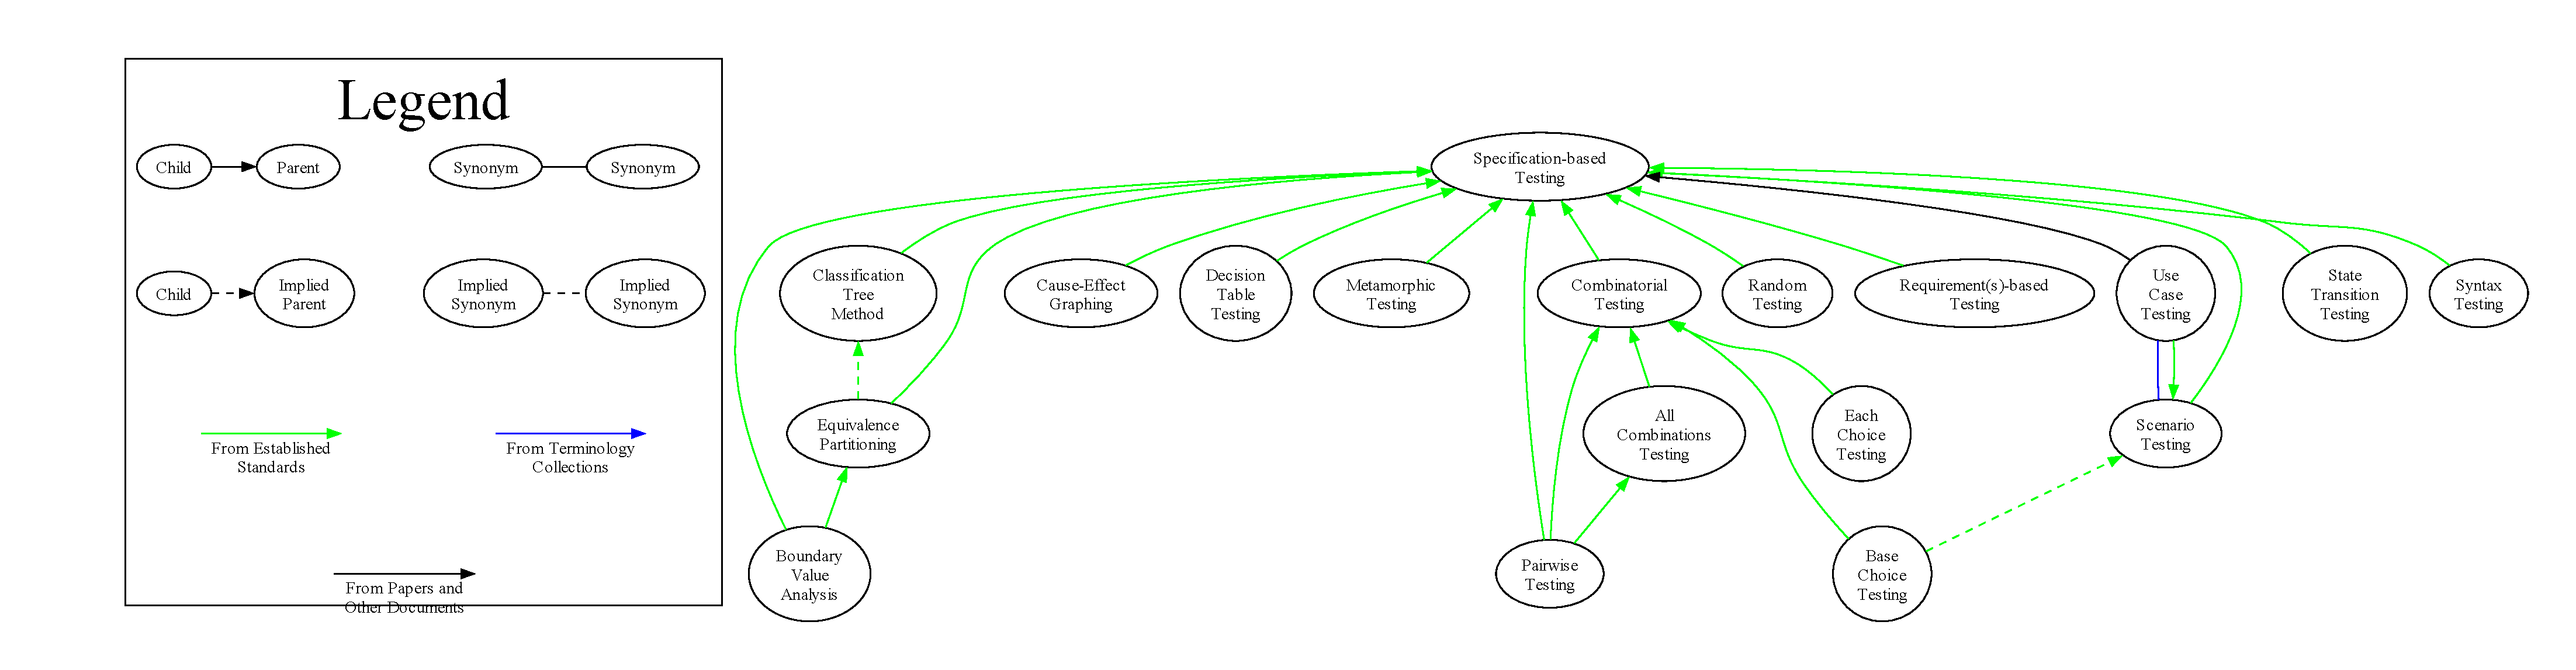
\includegraphics[width=\linewidth]{assets/graphs/specBasedGraph.pdf}
            \caption{``Superset'' relations.}
            \label{fig:specBasedGraph}
        \end{subfigure}
        \begin{subfigure}[t]{.45\linewidth}
            \centering
            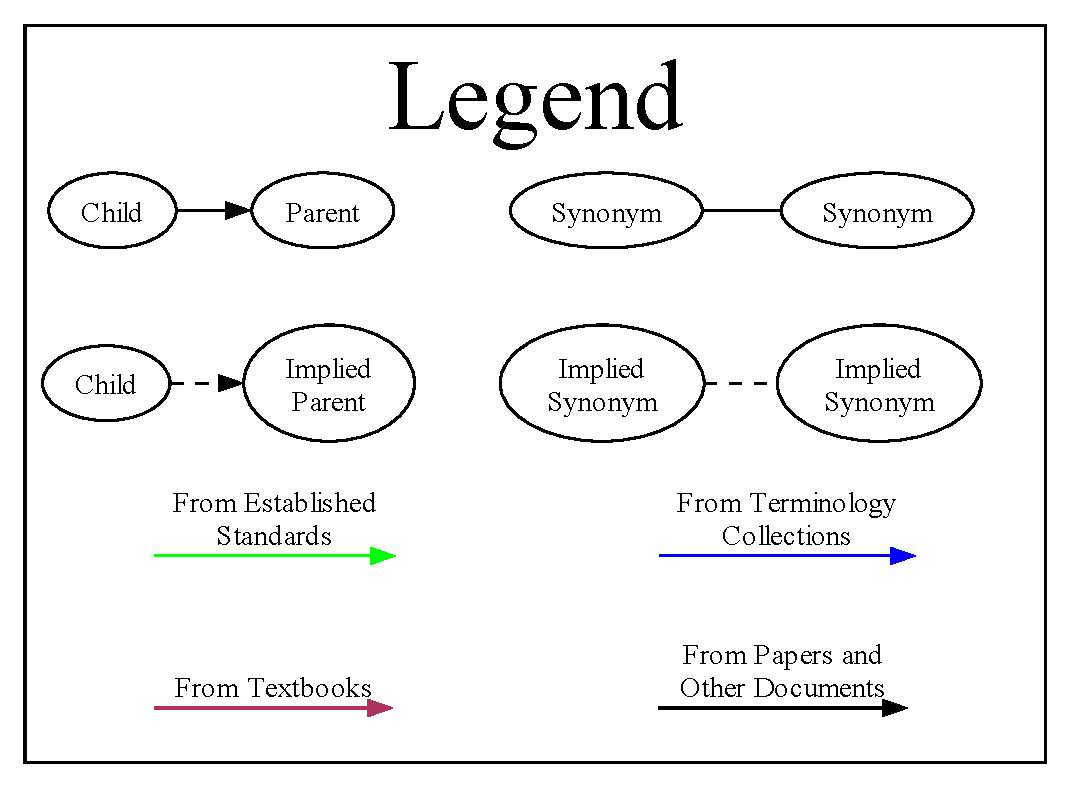
\includegraphics[width=\linewidth]{assets/graphs/parChdLegend.pdf}
        \end{subfigure}
        \begin{subfigure}[t]{.5\linewidth}
            \centering
            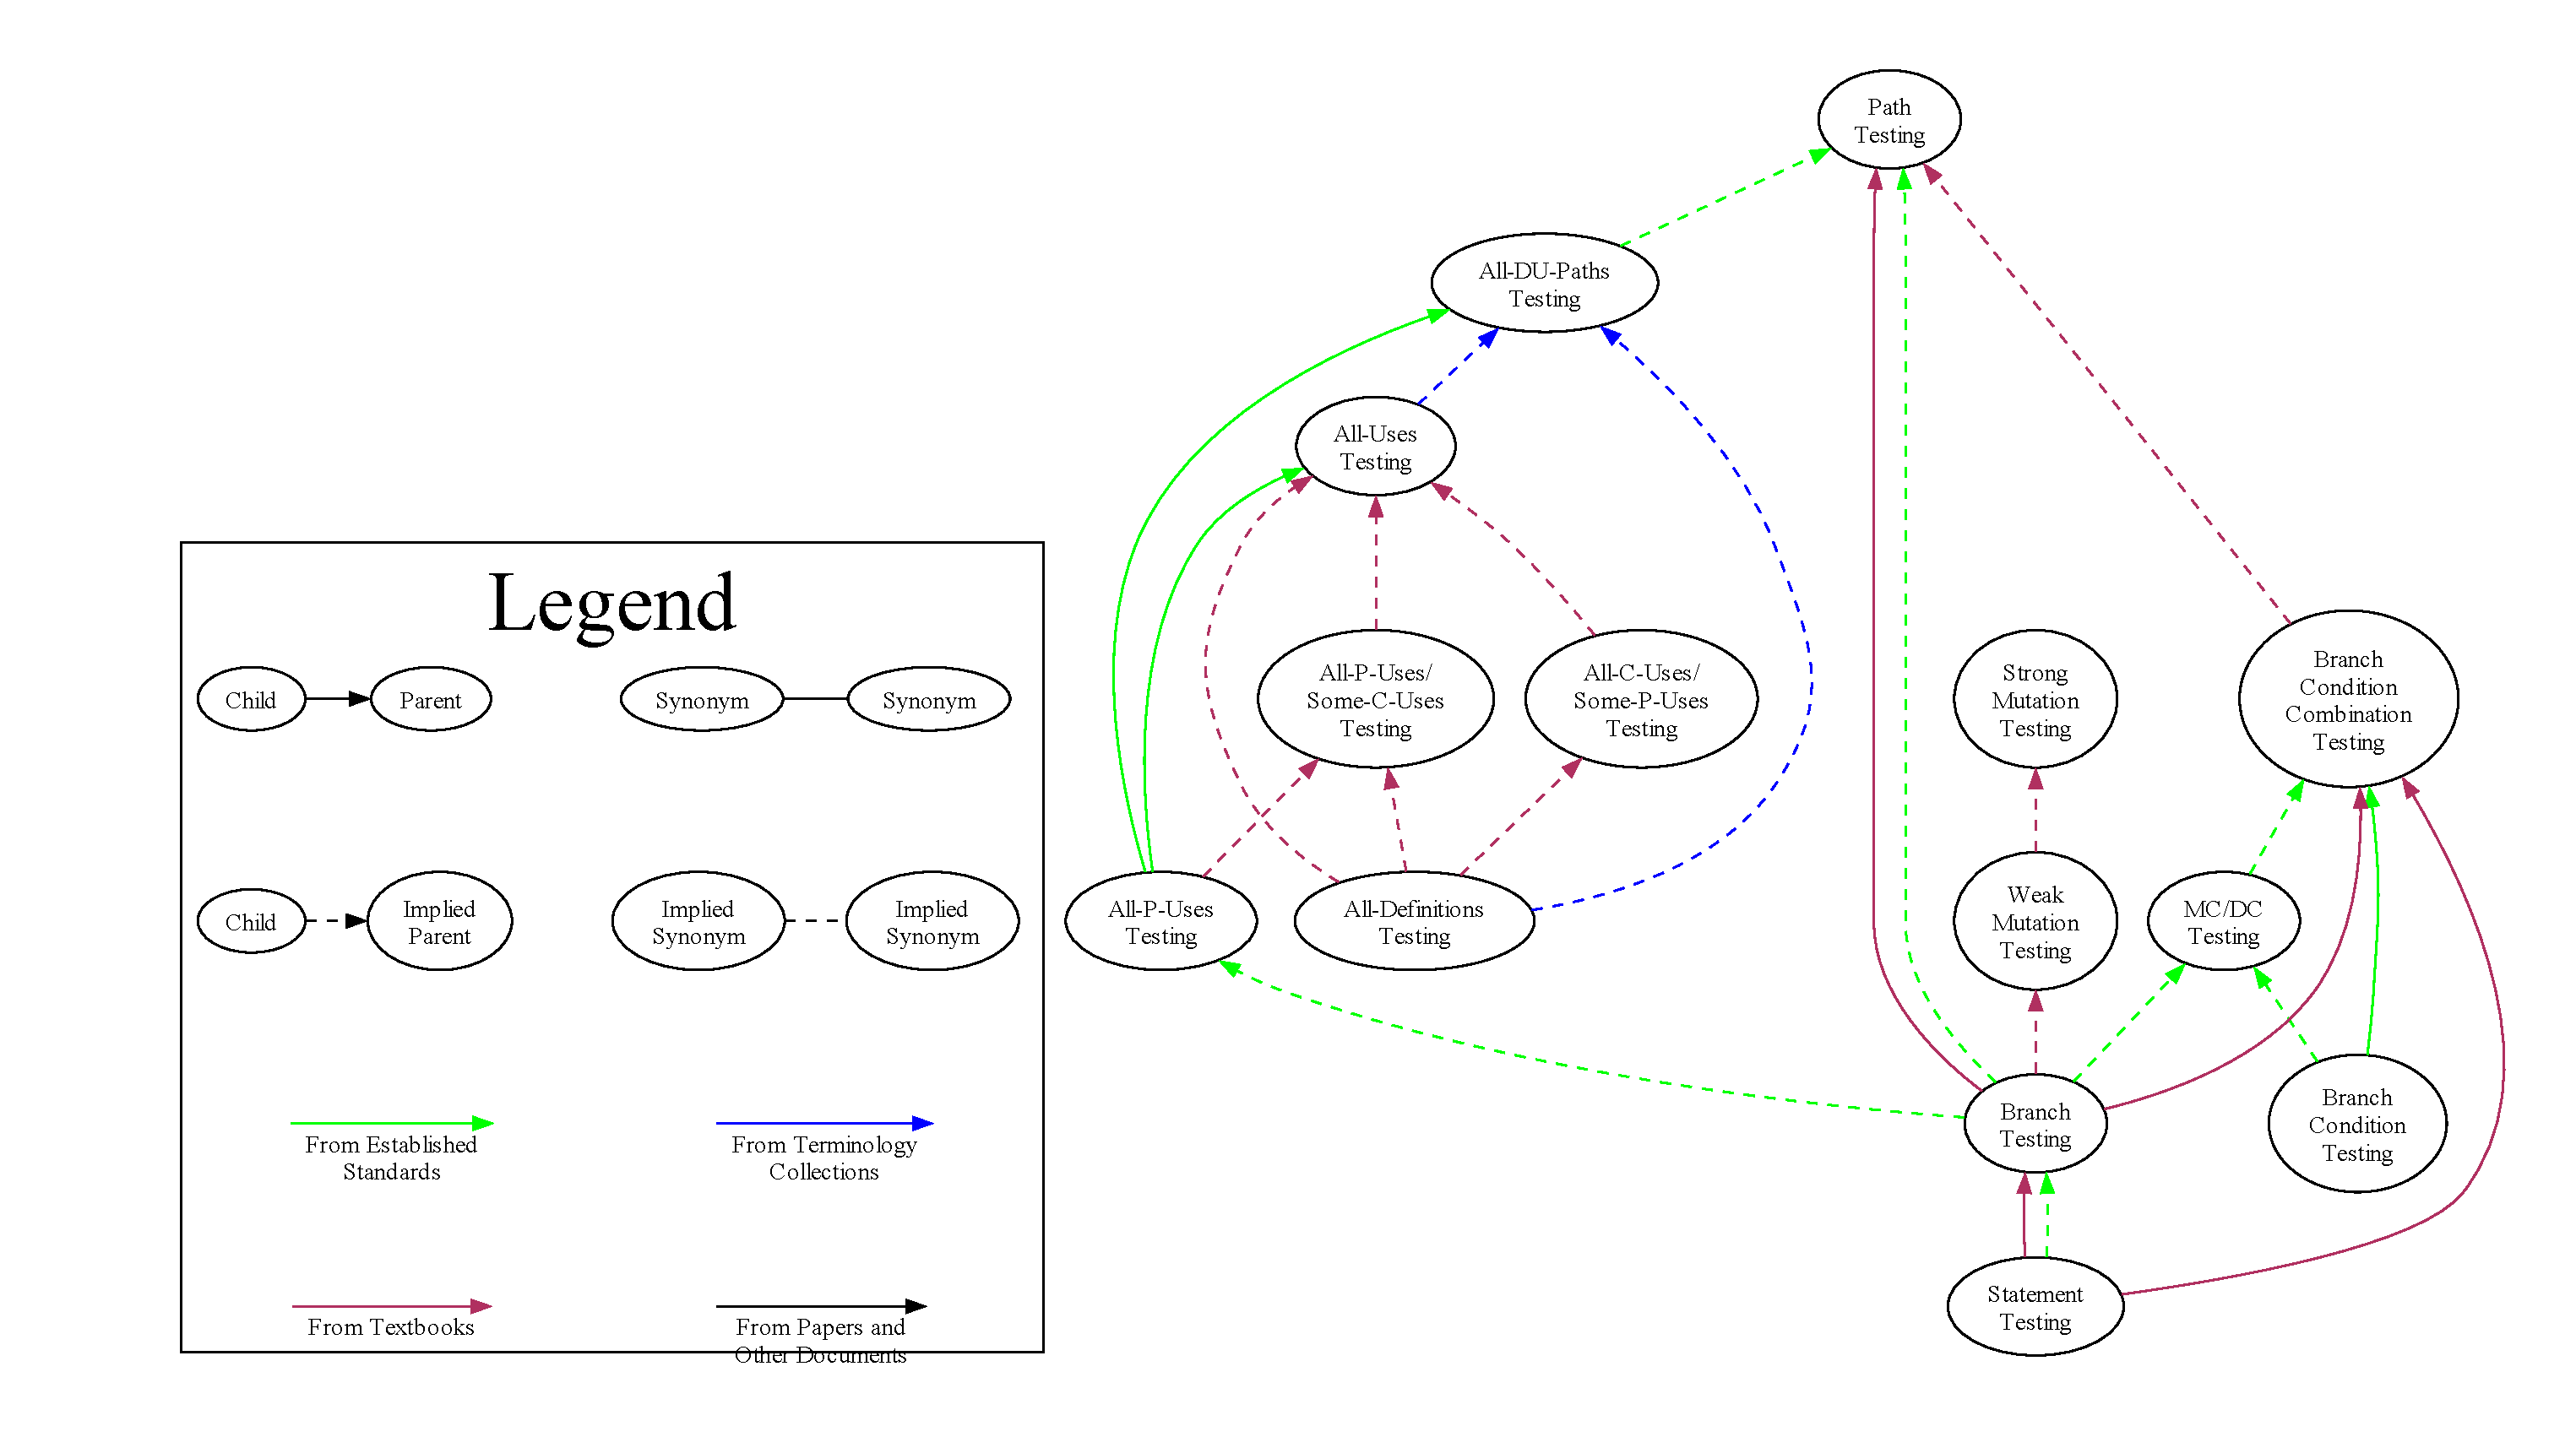
\includegraphics[width=\linewidth]{assets/graphs/subsumesGraph.pdf}
            \caption{``Subsume'' relations.}
            \label{fig:subsumesGraph}
        \end{subfigure}
        \caption{Graphs of different classes of \hyperref[par-chd-rels]{parent-child relations}.}
        \label{fig:parChdGraphs}
    \end{figure}
}

\newcommand{\ExampleGraph}{
    \begin{figure*}
        \begin{subfigure}[b]{0.3\linewidth}
            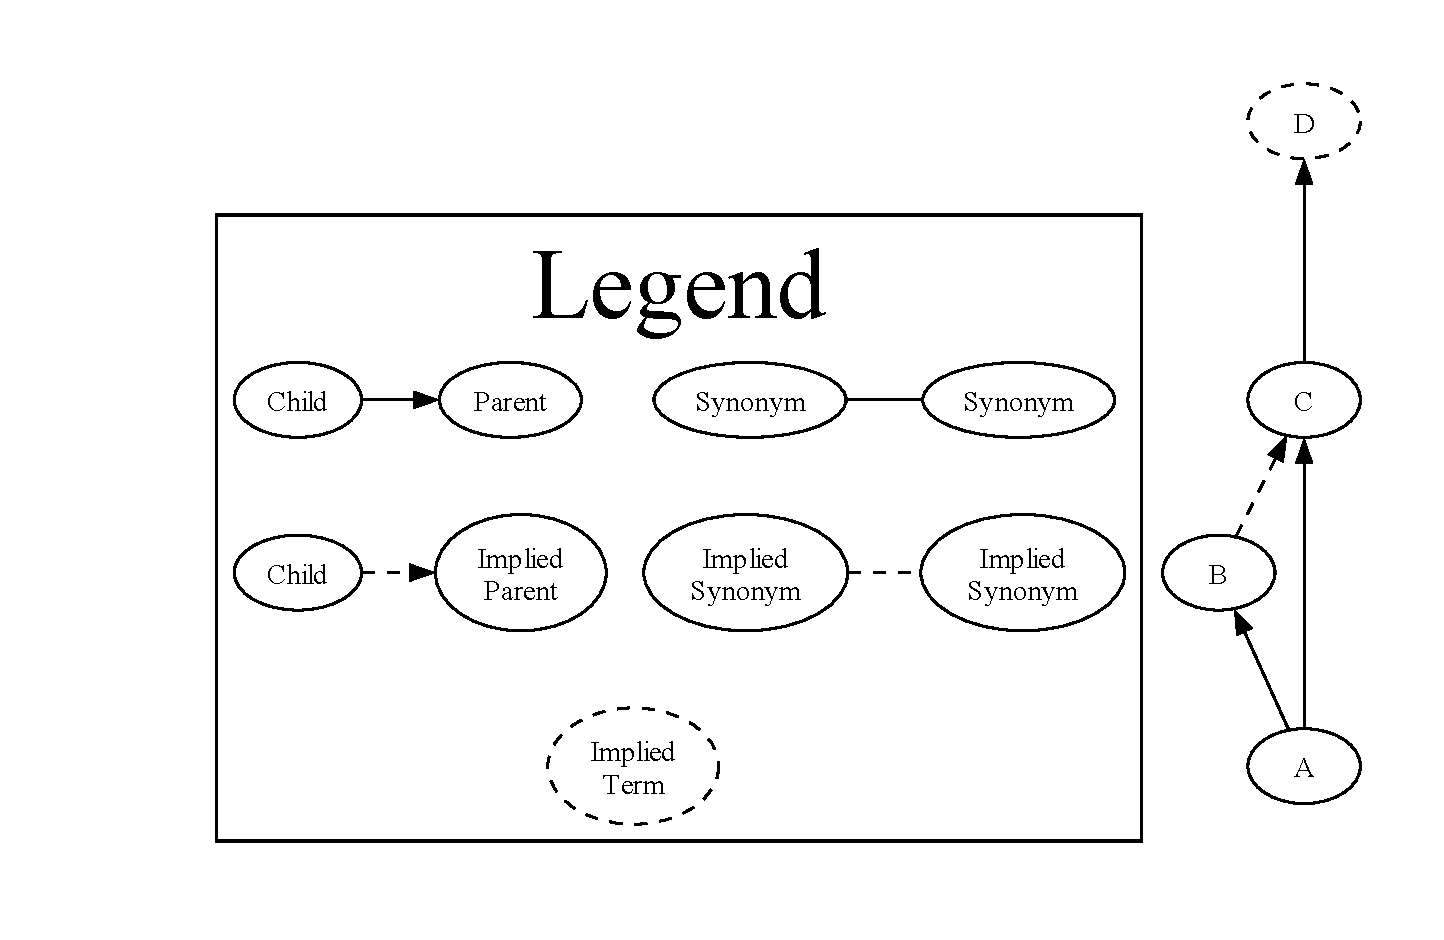
\includegraphics[width=\linewidth]{assets/graphs/ExampleGlossaryGraph.pdf}
            \caption{Graph from \Cref{tab:exampleGlossary}.}
            \label{fig:exampleGraph}
        \end{subfigure}
        \centering
        \begin{subfigure}[b]{0.675\linewidth}
            \centering
            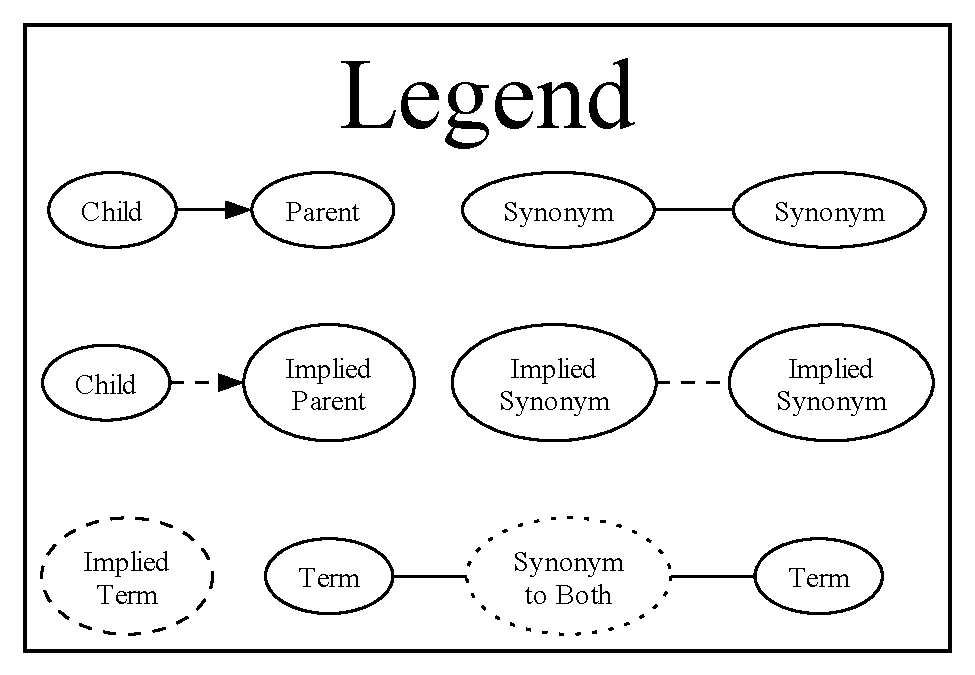
\includegraphics[width=0.8\linewidth]{assets/graphs/manual/manualLegendNonSolidTerms.pdf}
            \hspace{5cm}\begin{subfigure}[t]{0.475\linewidth}
                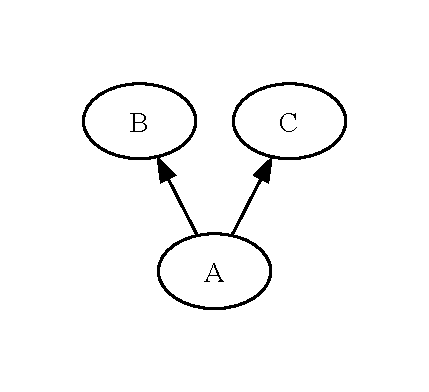
\includegraphics[width=1.1\linewidth]{assets/graphs/rigidExampleGlossaryGraph.pdf}
                \caption{Rigid graph from\\\Cref{tab:exampleGlossary}.}
                \label{fig:rigidExampleGraph}
            \end{subfigure}
            \begin{subfigure}[t]{0.475\linewidth}
                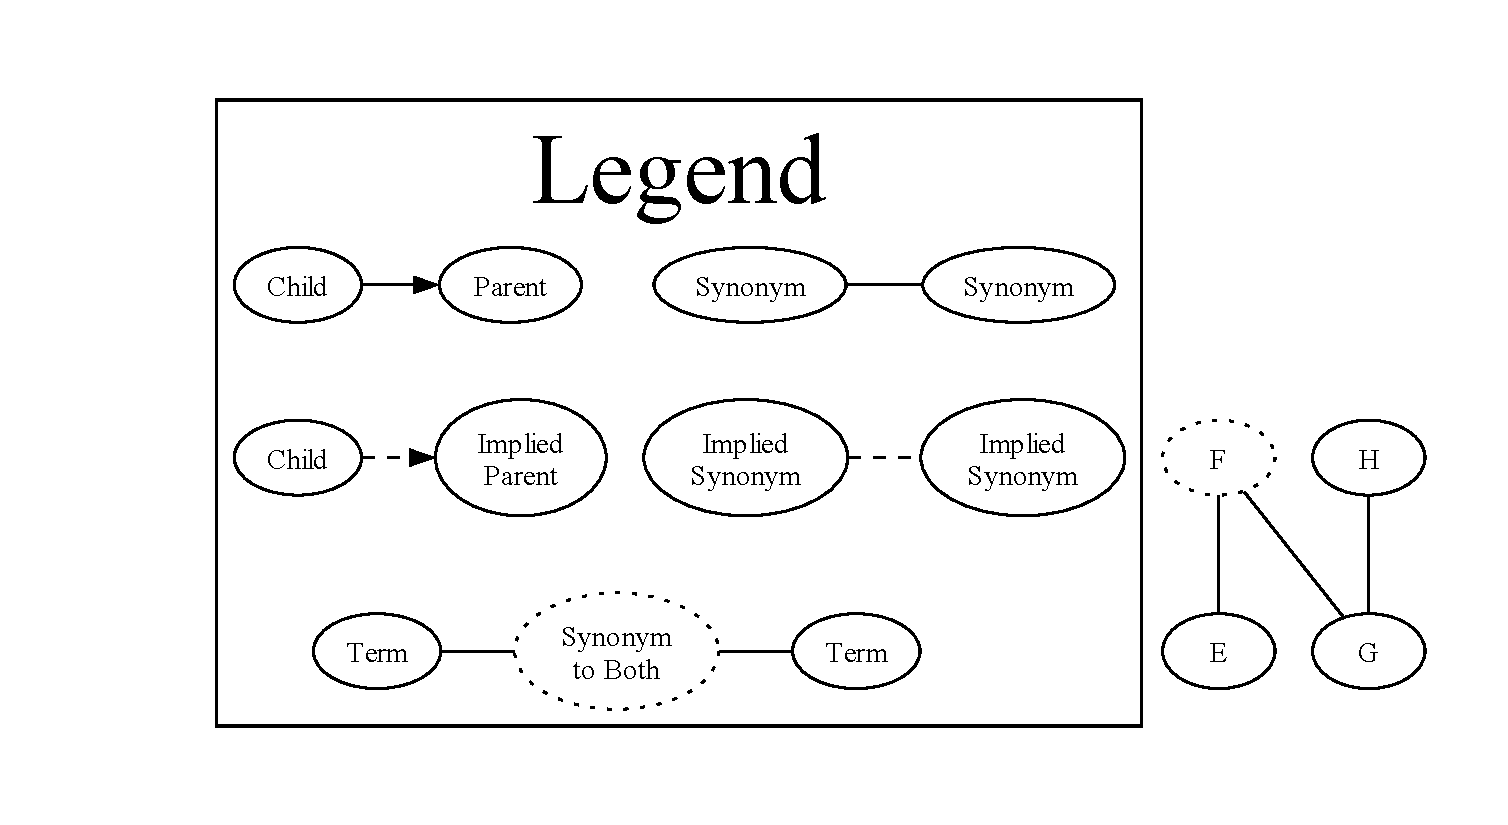
\includegraphics[width=1.1\linewidth]{assets/graphs/SynExampleGlossaryGraph.pdf}
                \caption{Graph from \Cref{tab:synExampleGlossary}.}
                \label{fig:synExampleGraph}
            \end{subfigure}
        \end{subfigure}
        \begin{subfigure}[t]{0.25\linewidth}
            \centering
            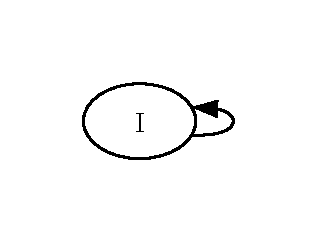
\includegraphics[width=1.2\linewidth]{assets/graphs/SelfExampleGlossaryGraph.pdf}
            \caption{Self-loop graph.}
            \label{fig:selfExampleGraph}
        \end{subfigure}
        \hfill
        \begin{subfigure}[t]{0.425\linewidth}
            \centering
            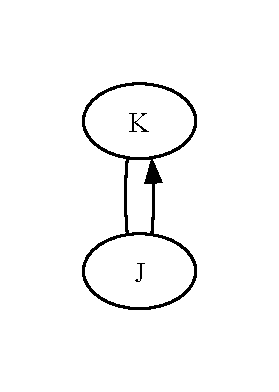
\includegraphics[width=0.6\linewidth]{assets/graphs/ParSynExampleGlossaryGraph.pdf}
            \caption{Graph of a pair of terms with a \hyperref[par-chd-rels]{parent-child} \emph{and} synonym relation.}
            \label{fig:parSynExampleGraph}
        \end{subfigure}
        \hfill
        \begin{subfigure}[t]{0.25\linewidth}
            \centering
            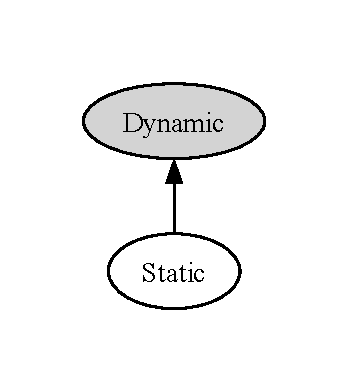
\includegraphics[width=1.4\linewidth]{assets/graphs/StaticExampleGlossaryGraph.pdf}
            \caption{Static graph.}
            \label{fig:staticExampleGraph}
        \end{subfigure}
        \caption{Example generated graphs.}
        \label{fig:exampleGraphs}
    \end{figure*}
}

\newcommand{\recoveryGraphs}{
    % Only top or bottom to comply with IEEE guidelines
    \begin{figure}[bt!]
        \centering
        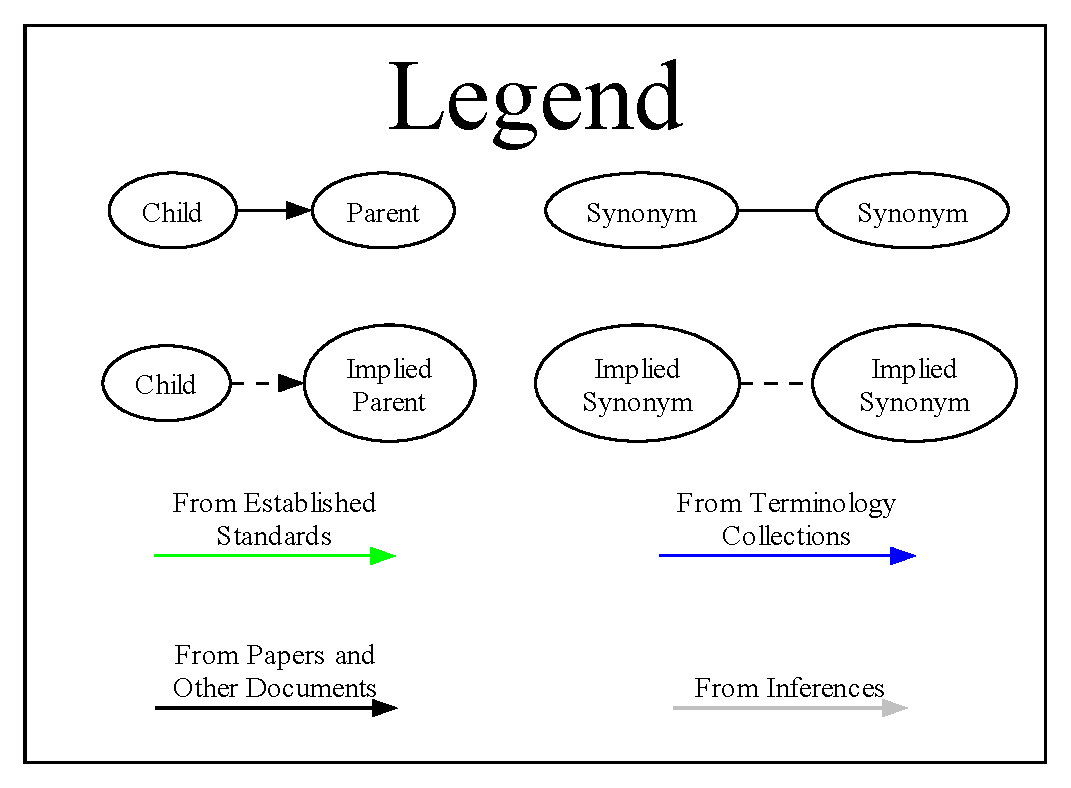
\includegraphics[width=\linewidth]{assets/graphs/recoveryLegend.pdf}
        \begin{subfigure}[b]{.55\linewidth}
            \centering
            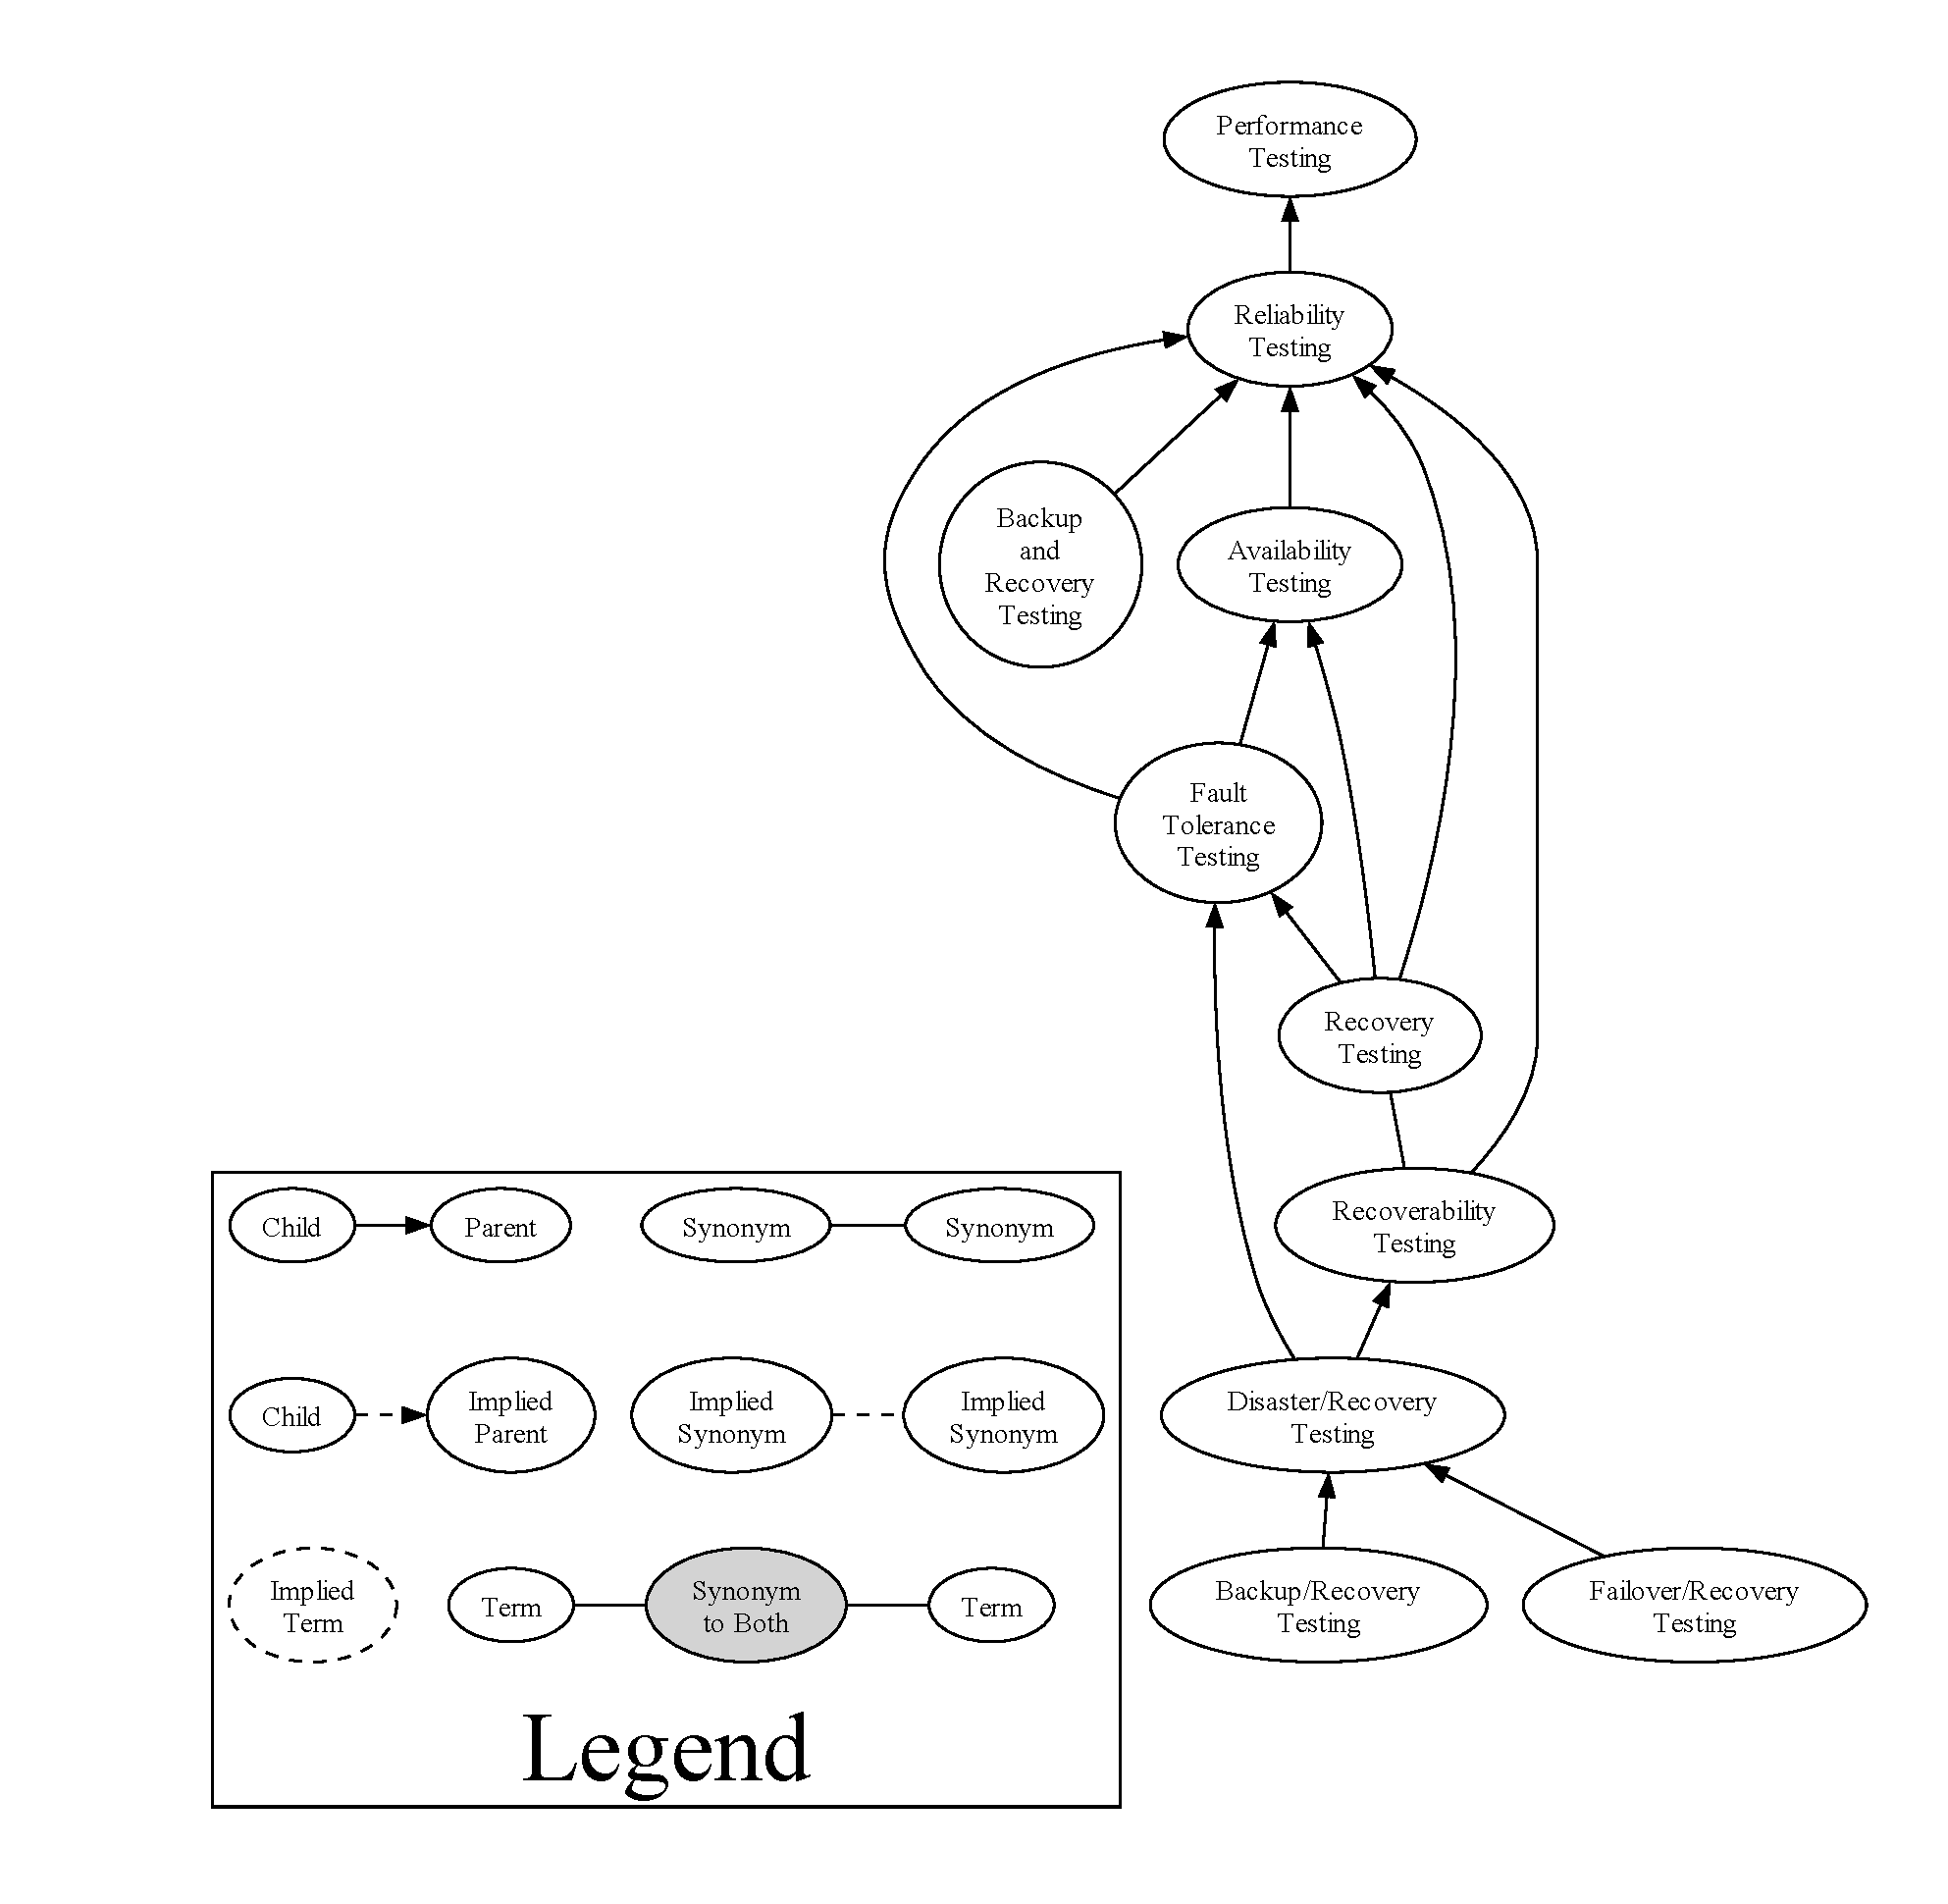
\includegraphics[width=\linewidth]{assets/graphs/recoveryGraph.pdf}
            \caption{Graph of current relations.}
            \label{fig:recovery-graph-current}
        \end{subfigure}
        \begin{subfigure}[b]{.4\linewidth}
            \centering
            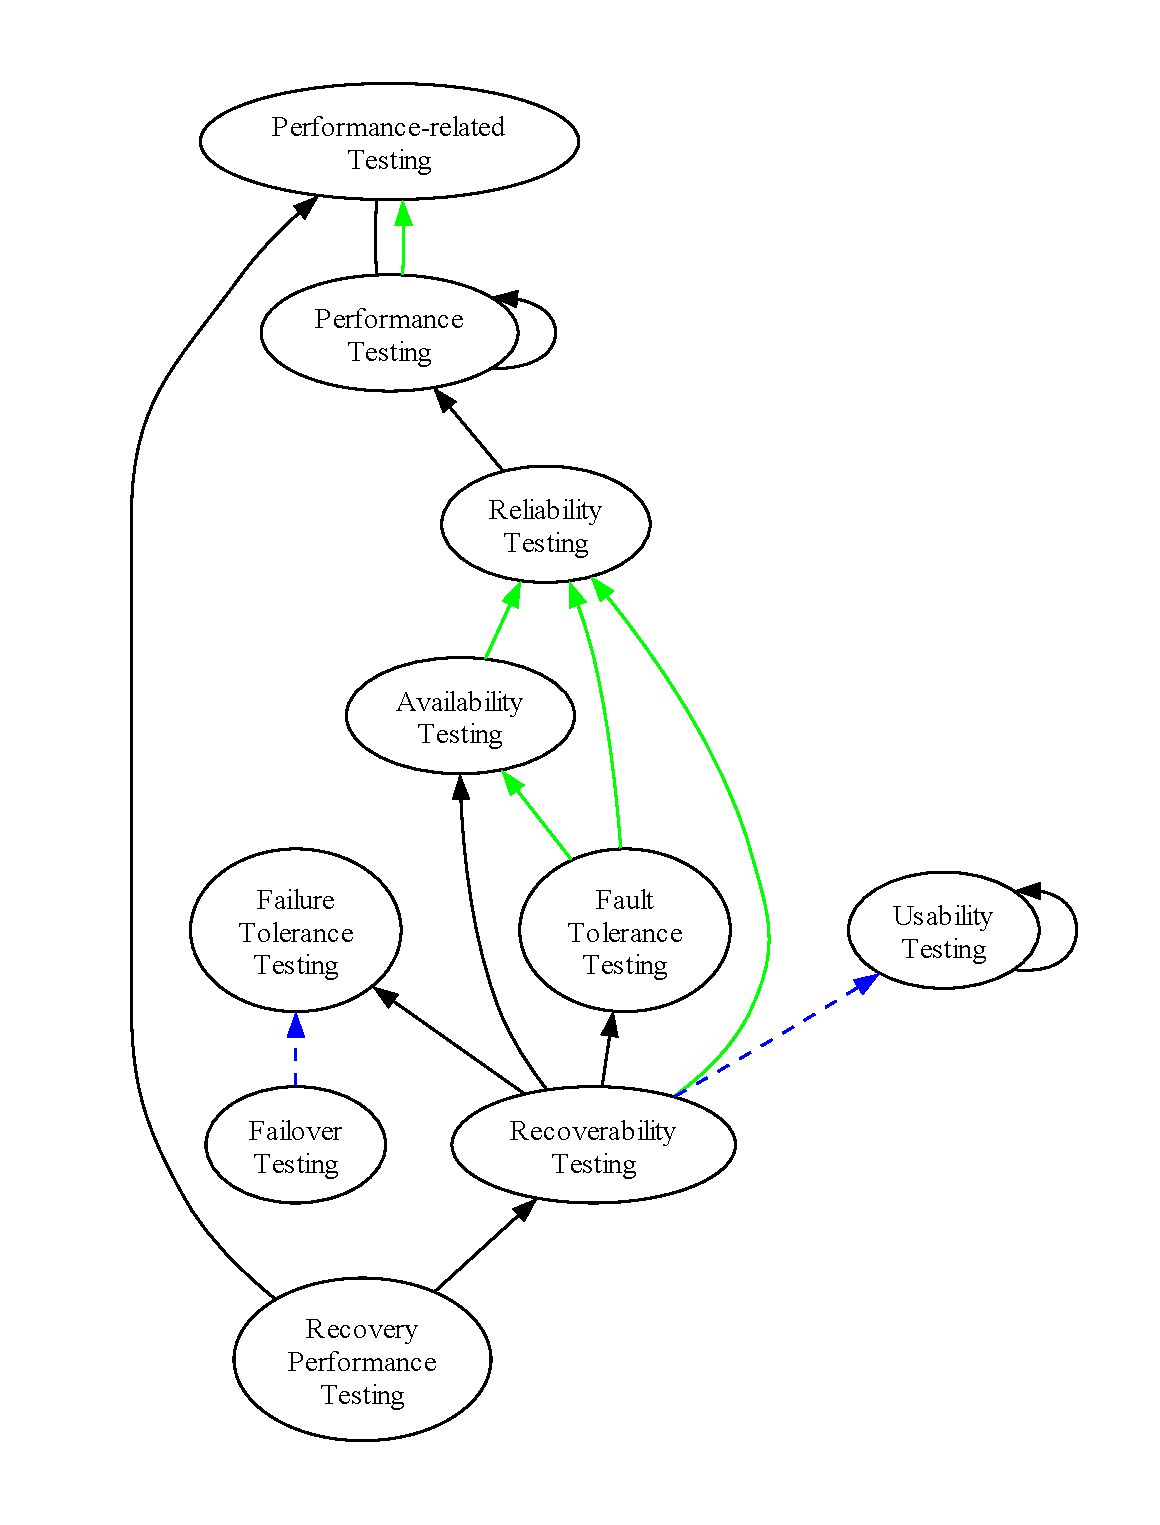
\includegraphics[width=\linewidth]{assets/graphs/recoveryProposedGraph.pdf}
            \caption{Graph of proposed relations.}
            \label{fig:recovery-graph-proposed}
        \end{subfigure}
        \caption{Graphs of relations between terms related to recovery testing.}
        \label{fig:recoveryGraphs}
    \end{figure}
}

\newcommand{\scalGraphs}{
    % Only top or bottom to comply with IEEE guidelines
    \begin{figure}[bt!]
        \centering
        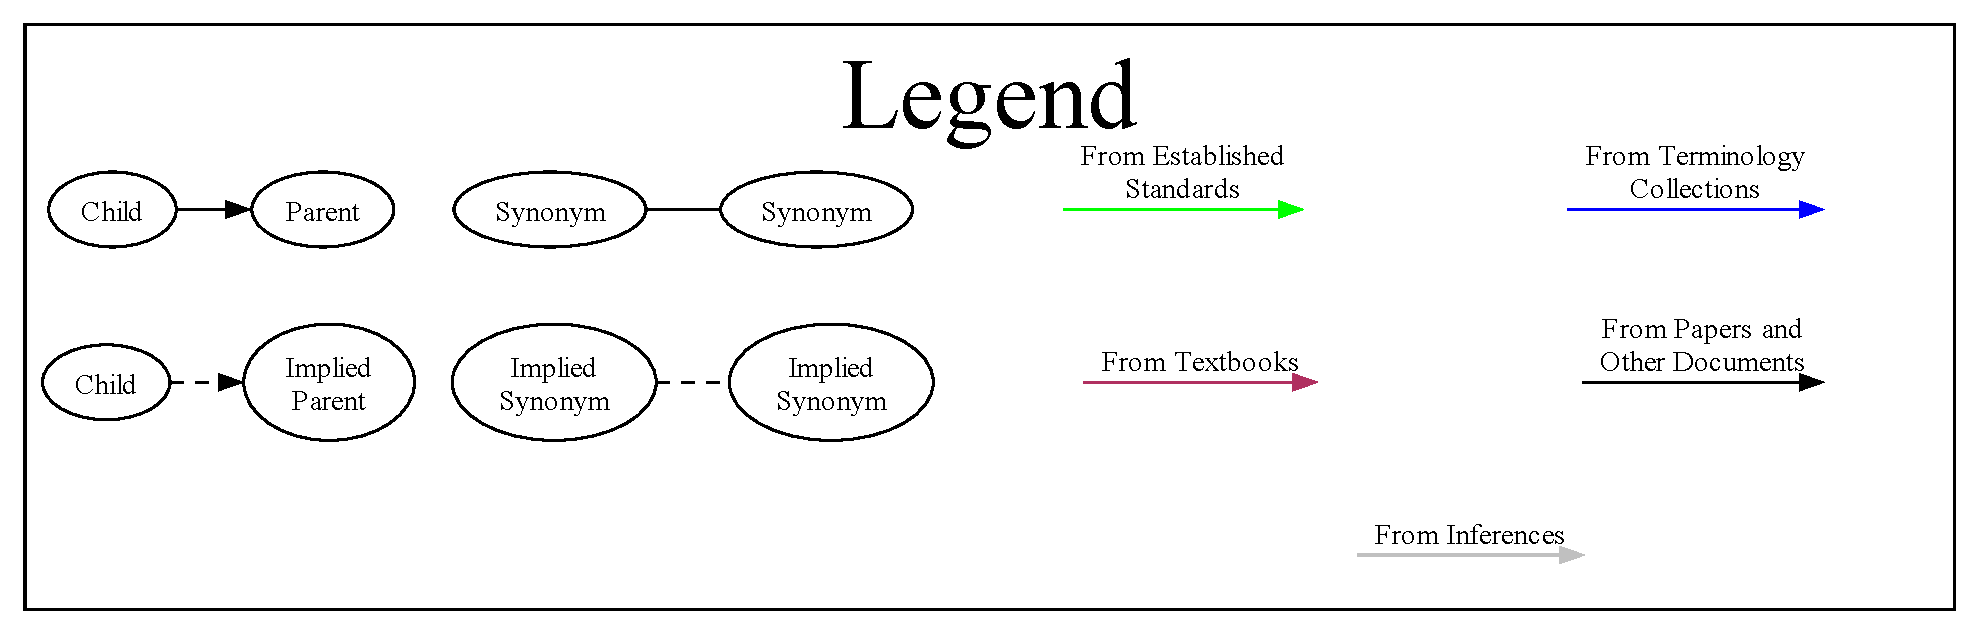
\includegraphics[width=\linewidth]{assets/graphs/scalabilityLegend.pdf}
        \begin{subfigure}[b]{.475\linewidth}
            \centering
            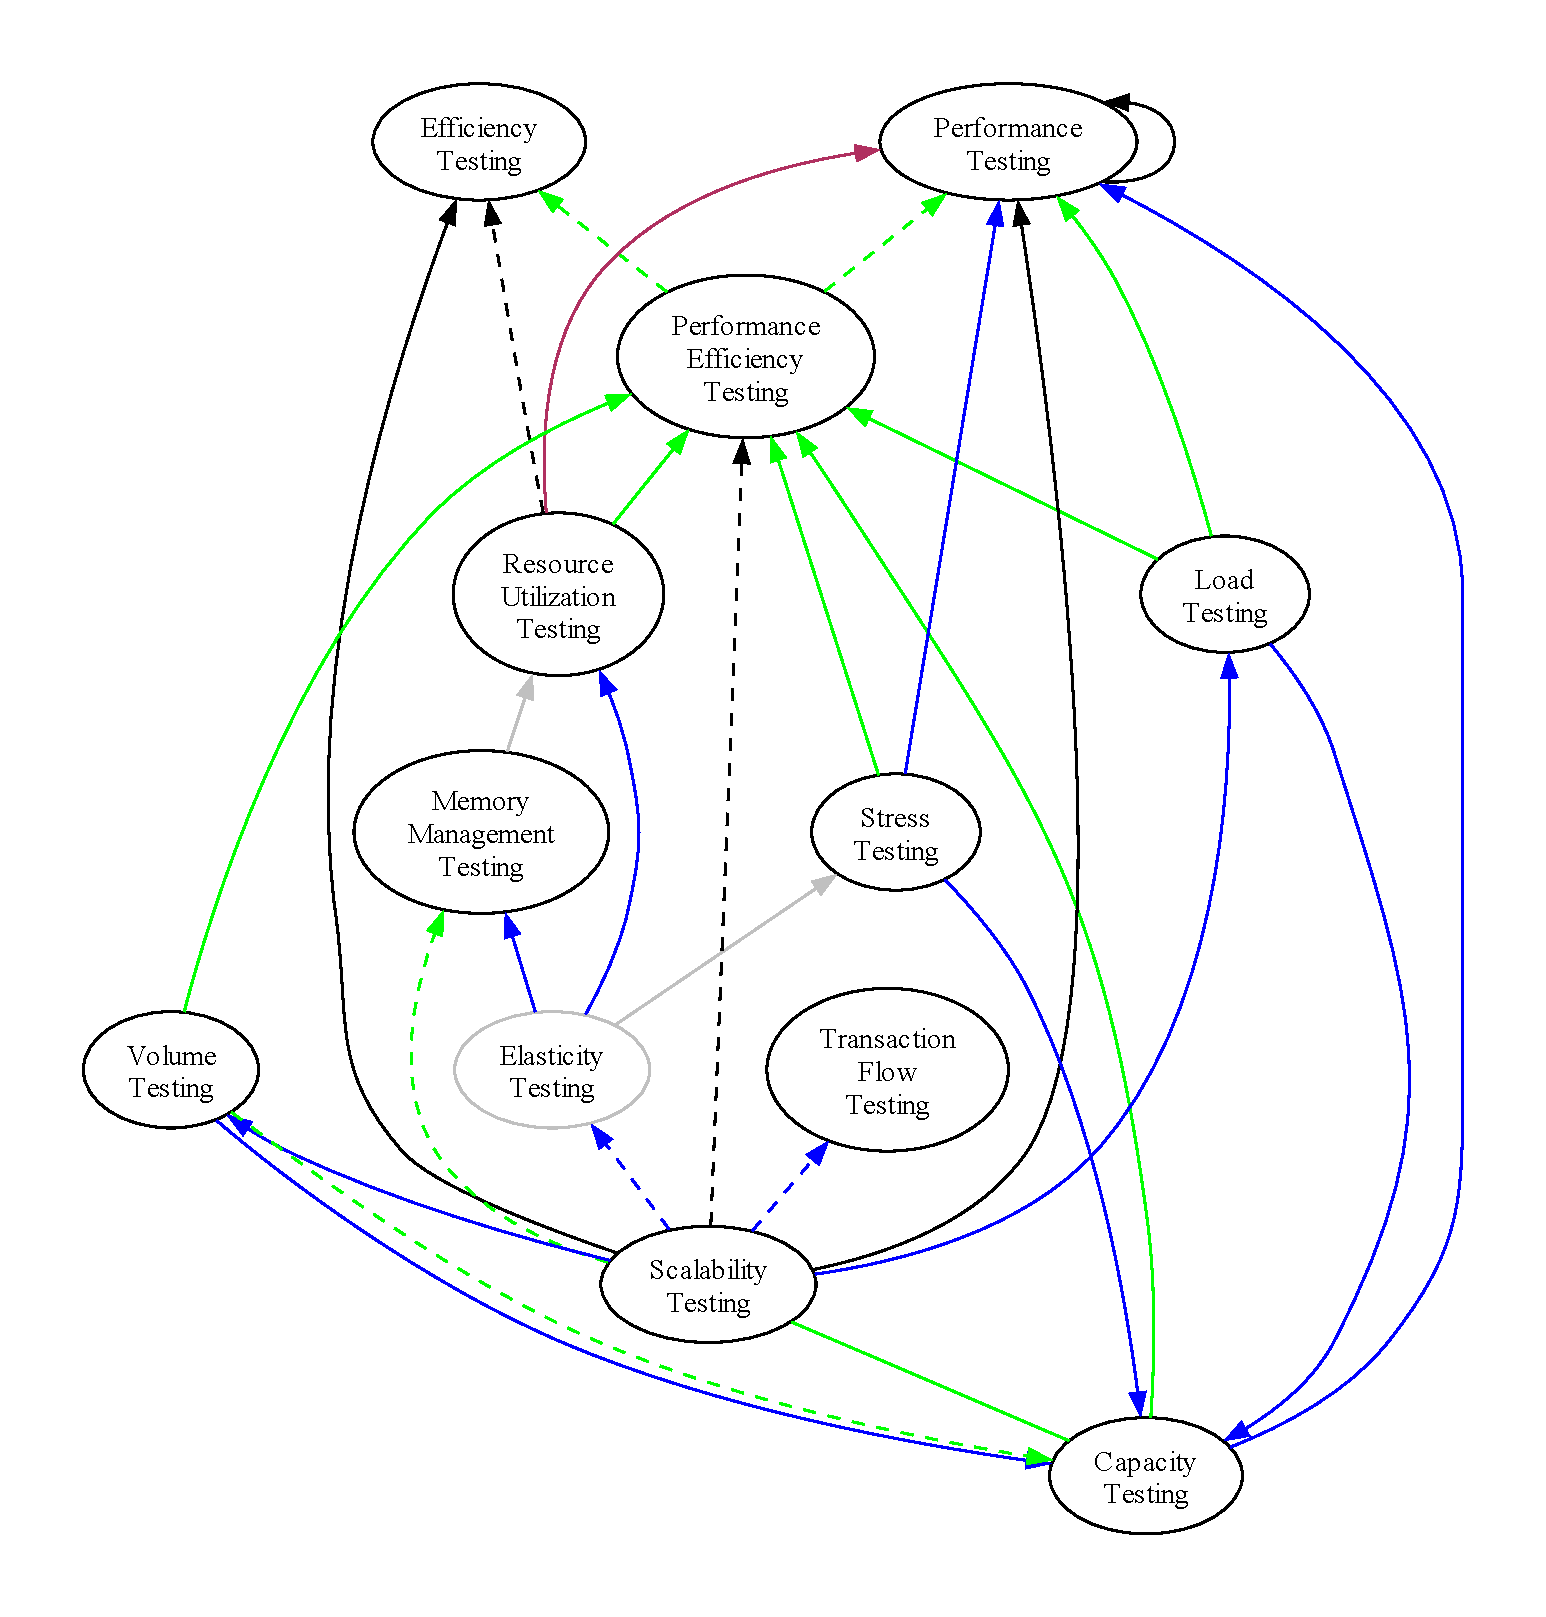
\includegraphics[width=\linewidth]{assets/graphs/scalabilityGraph.pdf}
            \caption{Graph of current relations.}
            \label{fig:scal-graph-current}
        \end{subfigure}
        \begin{subfigure}[b]{.475\linewidth}
            \centering
            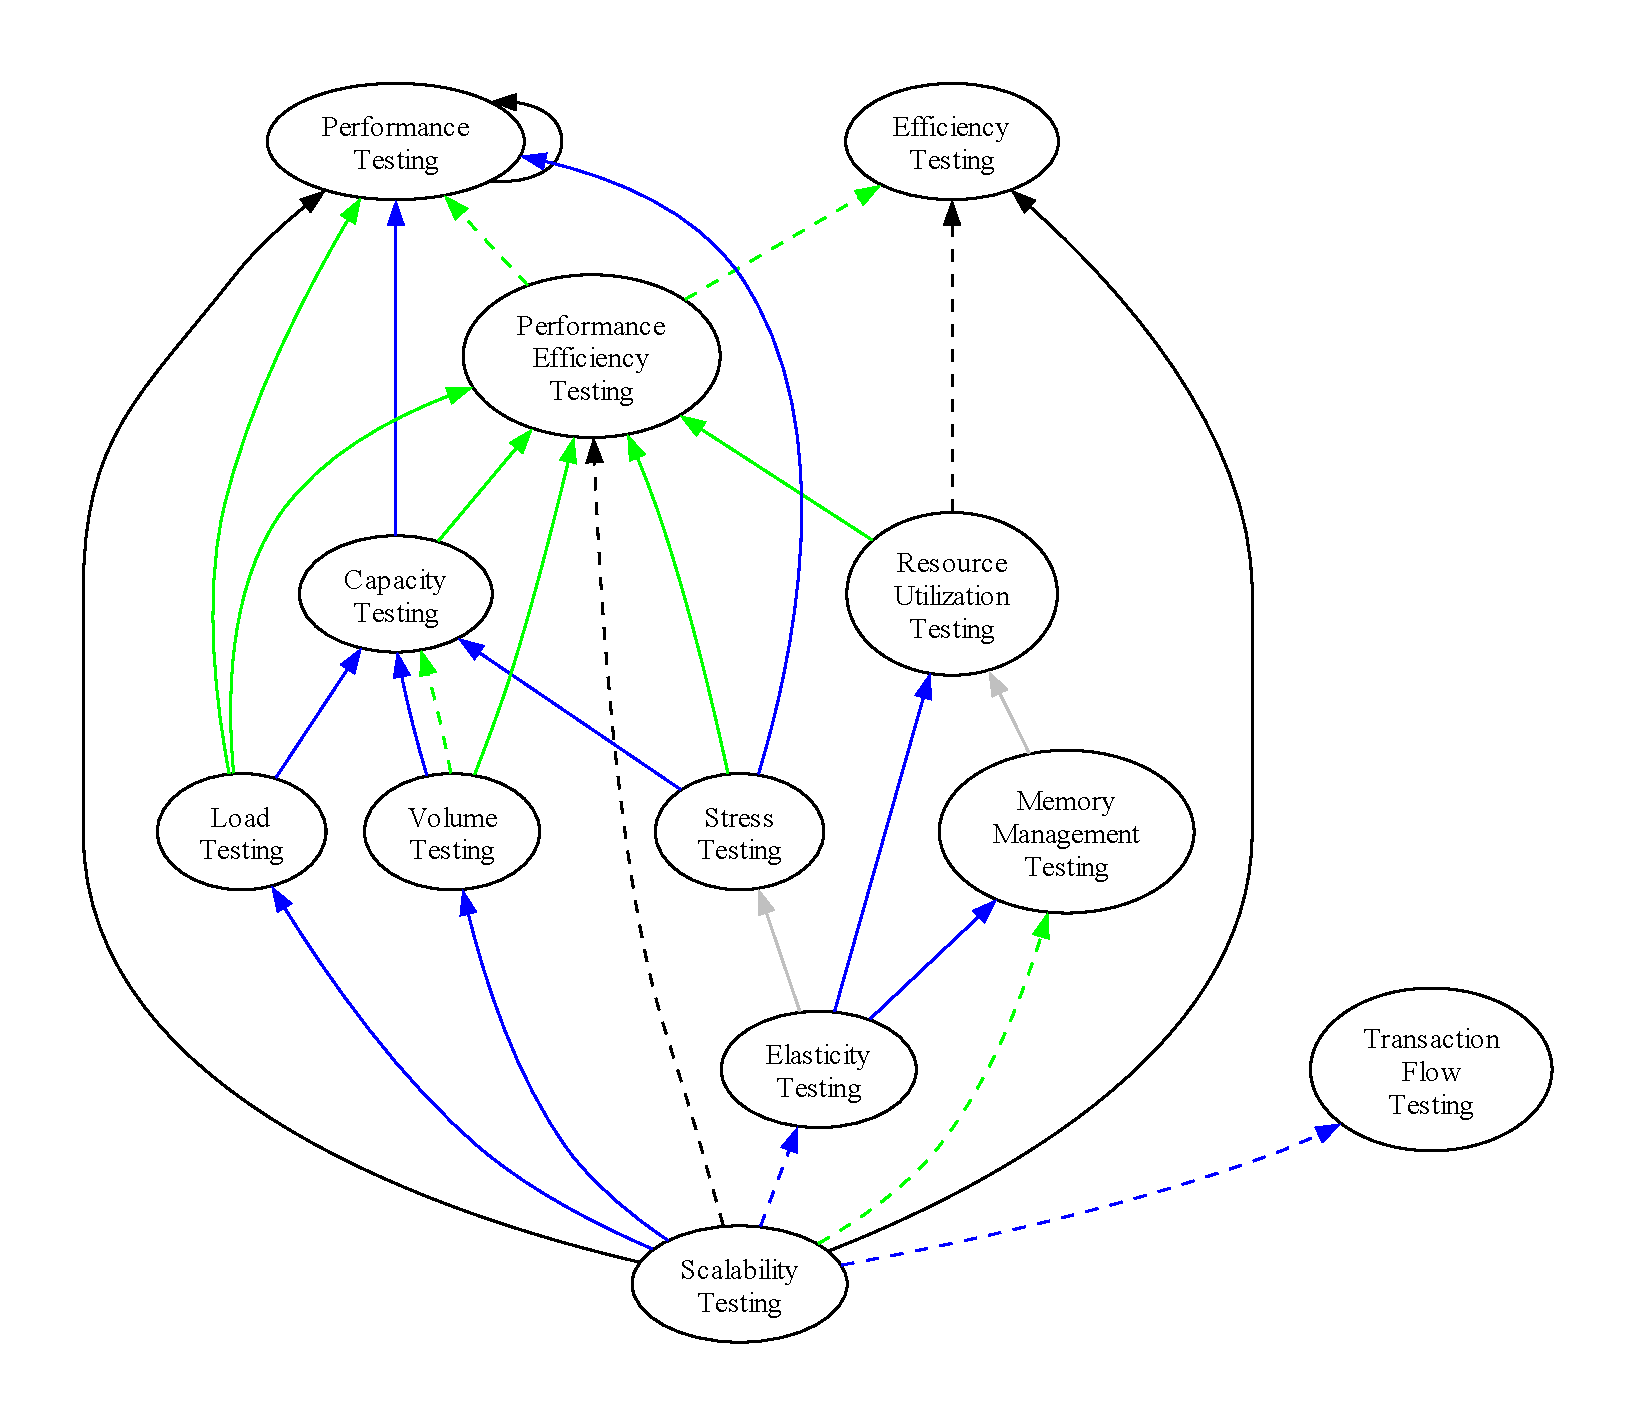
\includegraphics[width=\linewidth]{assets/graphs/scalabilityProposedGraph.pdf}
            \caption{Graph of proposed \ifnotpaper \else \\ \fi relations.}
            \label{fig:scal-graph-proposed}
        \end{subfigure}
        \caption{Graphs of relations between terms related to scalability testing.}
        \label{fig:scalGraphs}
    \end{figure}
}

\newcommand{\performanceGraph}{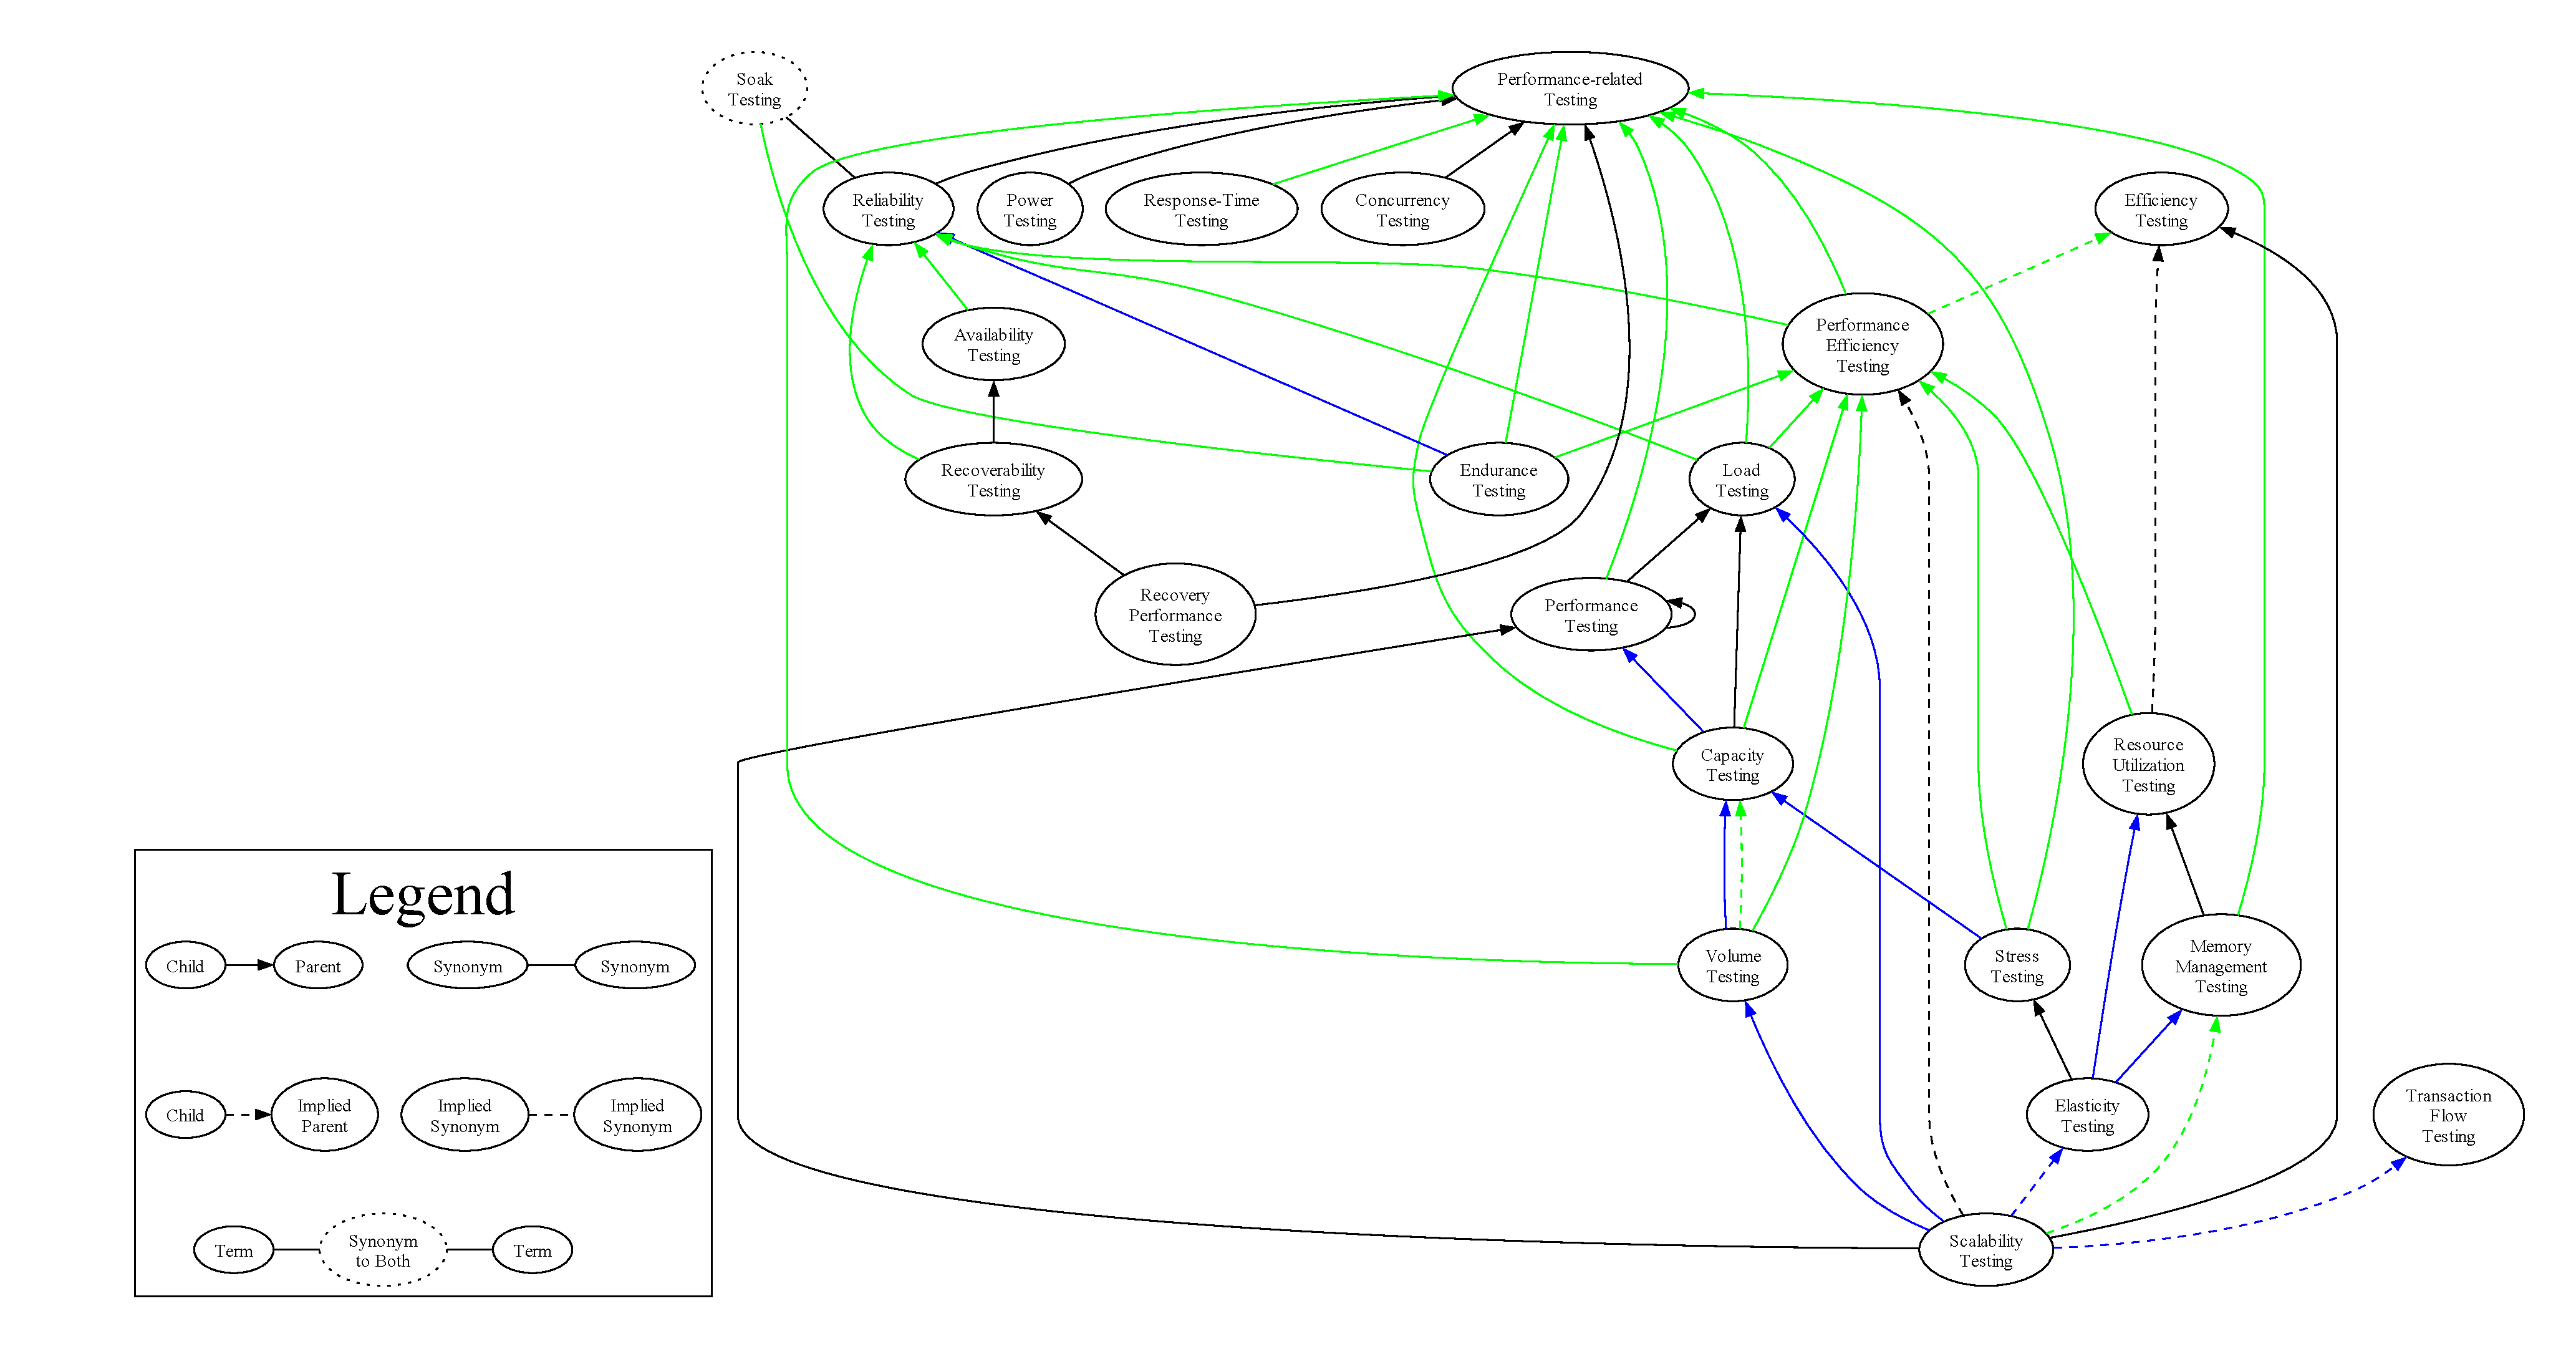
\includegraphics[width=\linewidth]{assets/graphs/performanceProposedGraph.pdf}}

%------------------------------------------------------------------------------
% Images & Figures
%------------------------------------------------------------------------------

\newcommand{\drasilLogo}{assets/images/drasil_logo.png}
\newcommand{\drasilLogoImg}{\begin{figure}[H]
    \centering
    \caption{Drasil's Logo}
    \label{fig:drasilLogo}

    \includegraphics[width=0.6\linewidth]{\drasilLogo}
\end{figure}
}
\newcommand{\refDrasilLogoImg}{\Cref{fig:drasilLogo}}

%------------------------------------------------------------------------------
% Tables
%------------------------------------------------------------------------------

% Organization of files
\newcommand{\organizationTable}{\begin{longtable}[c]{|>{\raggedright}p{0.3\linewidth}|>{\raggedright\arraybackslash}p{0.54\linewidth}|}
    \caption{Template Organization}
    \label{tab:organization}                                              \\

    \hline

    \rowcolor{McMasterMediumGrey}
    \textbf{File/Folder}     & \textbf{Intended Usage \& Description}
    \\ \hline

    \texttt{thesis.tex} & Focal \LaTeX{} file that collects everything and is
    used to build your thesis/report document.
    \\ \hline

    \texttt{Makefile} & A basic \texttt{Makefile} configuration. See
    \texttt{make help} for a list of helpful commands. \\ \hline

    \texttt{build/} & When you build your \acs{pdf}, this folder is used as the
    working directory of LuaLaTeX. Using this allows us to quickly get rid of
    \LaTeX{} build files that can cause problems when we re-build documents. \\
    \hline

    \texttt{manifest.tex} & Basic options that you should certainly configure
    according to your needs.
    \\ \hline

    \texttt{chapters.tex} & All chapters of your thesis should be included here.
    \\ \hline

    \texttt{chapters/} & Enumeration of the chapters of your thesis. I prefer
    using a two-digit indexing pattern for the prefix of file names so that I
    can quickly open up by chapter number using VS Codium. \\ \hline

    \texttt{assets.tex} & Enumeration of the various kinds of ``assets'' in the
    \texttt{assets/} folder. See the file for examples on how you can write your
    extra utility macros. \\ \hline

    \texttt{assets/} & Enumeration of various kinds of ``assets,'' with
    subdirectories for images and figures, tables, and code snippets. \\ \hline

    \texttt{front.tex} & All front matter of your thesis should be included
    here. \\ \hline

    \texttt{front/} & Enumeration of the front chapters of your thesis. These
    chapters should all be numbered using Roman numerals. \\ \hline

    \texttt{back.tex} & All back matter of your thesis should be included here.
    \\ \hline

    \texttt{back/} & Enumeration of the back matter content.
    \\ \hline

    \texttt{acronyms.tex} & List of acronyms you intend to use in your thesis.
    This uses the ``acro'' \LaTeX{} package.
    \\ \hline

    \texttt{macros.tex} & Helpful macros!
    \\ \hline

    \texttt{unicode\_chars.tex} & At times, you might find issues with unicode
    characters, especially in verbatim environments, where you might need to
    manually define them using other font glyphs.
    \\ \hline

    \texttt{mcmaster\_colours.tex} & Macros for the McMaster colour palette.
    \\ \hline

    \texttt{README.md} & Read it!
    \\ \hline

    \texttt{.gitignore} & List of files in the working directory that should be
    ignored by git.
    \\ \hline

    \texttt{latexmkrc} & Used for setting the timezone for latexmk, but can be
    used for other options.
    \\ \hline
\end{longtable}
}

\newcommand{\ieeeCatsTable}{% Conversion to longtblr assisted by GitHub Copilot

\begin{longtblr}[
    note{a} = {Also called ``test phase'' \ifnotpaper (see
            \discrepref{level-phase-syns}) \fi or ``test stage'' \ifnotpaper
            (see \discrepref{stage-level-syns})\else (see relevant synonym
            discrepancies in \Cref{syns})\fi.},
    note{b} = {Also called ``test design technique'' \ifnotpaper
            (\citealp[p.~11]{IEEE2022}; \citealpISTQB{})\else
            \cite[p.~11]{IEEE2022}, \cite{ISTQB}\fi.},
    caption={Categories of testing given by ISO/IEC and IEEE.},
    label={tab:ieeeCats}
    ]{
    colspec={|X[0.09,c,m]X[0.56,m]X[0.3,m]|},
    width = \linewidth, rowhead = 1, hlines
    }
    \thead{Term}                   & \thead{Definition}                           & \thead{Examples} \\
    Test Approach                  & A ``high-level test implementation choice''
    that includes ``test level, test type, test technique, test practice and
    \dots{} static testing'' \citep[p.~10]{IEEE2022} and is used to ``pick the
    particular test case values''
    \citeyearpar[p.~465]{IEEE2017} & black or white box, minimum and maximum
    boundary value testing \citep[p.~465]{IEEE2017}                                                  \\

    Test Level\TblrNote{a}         & A stage of testing ``typically associated
    with the achievement of particular objectives and used to treat particular
    risks'', each performed in sequence \ifnotpaper (\citealp[p.~12]{IEEE2022};
    \citeyear[p.~6]{IEEE2021}) \else \cite[p.~12]{IEEE2022}, \cite[p.~6]{IEEE2021}
    \fi with their ``own documentation and resources''
    \citeyearpar[p.~469]{IEEE2017} % ; more generally, ``designat[es] \dots\ the
    % coverage and detail'' \citeyearpar[p.~249]{IEEE2017} 
                                   & unit/component testing, integration testing,
    system testing, acceptance testing \ifnotpaper (\citealp[p.~12]{IEEE2022};
    \citeyear[p.~6]{IEEE2021}; \citeyear[p.~467]{IEEE2017}) \else
    \cite[p.~12]{IEEE2022}, \cite[p.~467]{IEEE2017}, \cite[p.~6]{IEEE2021} \fi                       \\
    Test Practice                  & A ``conceptual framework that can be
    applied to \dots{} [a] test process to facilitate testing'' \ifnotpaper
    (\citealp[p.~14]{IEEE2022}; \citeyear[p.~471]{IEEE2017}; OG IEEE 2013)
    \else \cite[p.~14]{IEEE2022}, \cite[p.~471]{IEEE2017}
    \fi % ; more generally, a ``specific type of activity that contributes to
    % the execution of a process'' \citeyearpar[p.~331]{IEEE2017} 
                                   & scripted testing, exploratory testing,
    automated testing \citep[p.~20]{IEEE2022}                                                        \\
    Test Technique\TblrNote{b}     & A ``procedure used to create or select a
    test model, identify test coverage items, and derive corresponding test
    cases'' \ifnotpaper (\citeyear[p.~11]{IEEE2022}; similar in
    \citeyear[p.~467]{IEEE2017}) \else \cite[p.~11]{IEEE2022} (similar in
    \cite[p.~467]{IEEE2017}) \fi that ``generate evidence that test item
    requirements have been met or that defects are present in a test item''
    \citeyearpar[p.~vii]{IEEE2021} % ; ``a variety \dots\ is typically
    % required to suitably cover any system'' \citeyearpar[p.~33]{IEEE2022} and
    % is ``often selected based on team skills and familiarity, on the format
    % of the test basis'', and on expectations \citeyearpar[p.~23]{IEEE2022}
                                   & equivalence partitioning,
    boundary value analysis, branch testing \citep[p.~11]{IEEE2022}                                  \\
    Test Type                      & ``Testing that is focused on specific
    quality characteristics'' \ifnotpaper (\citealp[p.~15]{IEEE2022};
    \citeyear[p.~7]{IEEE2021}; \citeyear[p.~473]{IEEE2017}; OG IEEE 2013)
    \else \cite[p.~15]{IEEE2022}, \cite[p.~473]{IEEE2017}, \cite[p.~7]{IEEE2021}
    \fi                            & security testing, usability testing,
    performance testing \ifnotpaper (\citealp[p.~15]{IEEE2022};
    \citeyear[p.~473]{IEEE2017}) \else\cite[p.~15]{IEEE2022},
    \cite[p.~473]{IEEE2017} \fi                                                                      \\
\end{longtblr}
}
\newcommand{\otherCatsTable}{% Defined here so VS Code doesn't freak out
\def\ieeeEquiv{\makecell{IEEE\\Equivalent}}
\def\swebokLevel{{Level\\(objective-\\based)\TblrNote{a}}}

\begin{longtblr}[
    note{a} = {See \flawref{stage-level-syns}.},
    note{b} = {Testing methods and guidances are omitted from this table
            since \citet{BarbosaEtAl2006} do not define or give examples of them.},
    note{c} = {Synonyms for these examples are used by
            \citet[p.~3; OG Mathur, 2012]{SouzaEtAl2017} and
            \citet[p.~3]{BarbosaEtAl2006}.},
    caption={Categories of testing given by other sources.},
    label={tab:otherCats}
    ]{
    colspec={|X[0.08,c,m]|X[0.43,m]|X[0.34,m]|Q[c,m]|},
    width = \linewidth, rowhead = 1
    }
    \hline
    \thead{Term}                           & \thead{Definition}           & \thead{Examples} & \thead{\ieeeEquiv{}} \\
    \hline
    % Guidance                               & none given
    % \citep[p.~3]{BarbosaEtAl2006}          & none given         & Technique?                              \\
    \swebokLevel{}                         & Test levels based on the
    purpose of testing \citep[p.~5\=/6]{SWEBOK2024} that ``determine
    how the test suite is identified \dots\ regarding its consistency
    \dots\ and its composition''
    \citetext{p.~5\=/2}                    & conformance testing,
    installation testing, regression testing, performance testing,
    security testing % reliability testing,
    \citep[pp.~5\=/7 to 5\=/9]{SWEBOK2024} & Type?                                                                  \\
    % Method                                 & none given
    % \citep[p.~3]{BarbosaEtAl2006}          & none given         & Practice?                               \\
    Phase                                  & none given
    %(\citealp[p.~221]{Perry2006}; \citealp[p.~3]{BarbosaEtAl2006})  
                                           & unit testing,
    integration testing, system testing, regression testing (\citealp[p.~221]{Perry2006};
    \citealp[p.~3]{BarbosaEtAl2006})       & Level                                                                  \\
    Procedure                              & The basis for how
    testing is performed that guides the process; ``categorized in[to] testing methods,
    testing guidances\TblrNote{b} and testing techniques''
    \citep[p.~3]{BarbosaEtAl2006}          & none given
    generally; see ``Technique''           & Approach                                                               \\
    Process                                & ``A sequence of
    testing steps'' \citep[p.~2]{BarbosaEtAl2006} ``based on a development technology and \dots\
    paradigm, as well as on a testing procedure''
    \citetext{p.~3}                        & none given                   & Practice                                \\
    Stage                                  & An
    alternative to the ``traditional \dots\ test stages'' %\footnote{See ``Level'' in \Cref{tab:ieeeCats}.}
    based on ``clear technical groupings''
    \citep[p.~13]{Gerrard2000a}            & desktop development testing,
    infrastructure testing,
    % system testing, large scale integration, and
    post-deployment monitoring
    \citep[p.~13]{Gerrard2000a}            & Level                                                                  \\
    Technique                              & ``Systematic
    procedures and approaches for generating or selecting the most suitable test suites''
    \citep[p.~5\=/10]{SWEBOK2024}          & specification-based testing,
    % ``on a sound theoretical basis'' \citep[p.~3]{BarbosaEtAl2006}
    structure-based testing, fault-based testing\TblrNote{c}
    % , experience-based testing, usage-based testing
    (\citealp[pp.~5\=/10, 5\=/13 to 5\=/15]{SWEBOK2024})
    % black-box, white-box, defect/fault-based, model-based testing
    % \citetext{\citealp[p.~3]{SouzaEtAl2017}; OG Mathur, 2012};
    % functional, structural, error-based, state-based testing \citep[p.~3]{BarbosaEtAl2006}
                                           & Technique                                                              \\
    \hline
\end{longtblr}
}
\newcommand{\otherCategorizationsTable}{\def\selecExs{Deterministic Testing\\ Random Testing}
\def\covExs{Input Space Partitioning\\ Graph Coverage\\ Logic Coverage\\ Syntax-based Testing}
\def\execExs{Static Testing\\ Dynamic Testing}
\def\goalExs{Verification Testing\\ Validation Testing}
\def\propExs{Functional Testing\\ Non-functional Testing}

\begin{paperTable}
    \centering
    \begin{minipage}{\linewidth}
        \begin{longtblr}[
            note{\textrm{a}} = {We also consider this categorization meaningful (see \Cref{static-test}).},
            note{\textrm{b}} = {Functional testing is categorized ambiguously (see \Cref{func-test-discrep}) and non-functional testing is uncategorized.},
            caption = {Alternate categorizations given by the literature.},
            label = {tab:otherCategorizations}
            ]{
            colspec = {|X[0.35,c,m]X[0.2,c,m]X[0.35,c,m]|}, width = \linewidth,
            rowhead = 1
            }
            \hline
            \thead{Test Basis}                                        & \thead{Example Approaches} & \thead{Subset of}                                                                                                                      \\
            \hline
            Selection Process \citep[p.~5-16]{SWEBOK2024}             & \selecExs{}                & Technique \citep[pp.~5-12, 5-16]{SWEBOK2024}                                                                                           \\
            \hline
            Coverage Criteria \citep[pp.~18--19]{AmmannAndOffutt2017} & \covExs{}                  & Technique (\citealp[p.~22]{IEEE2022}; \citeyear[Fig.~2]{IEEE2021}; \citealp[p.~5-11]{SWEBOK2024}; \citealp[pp.~47--48]{Firesmith2015}) \\
            \hline
            Execution of Code{\MidTblrNote{\textrm{a}}} (\citealp[p.~214]{KuļešovsEtAl2013}; \citealp[p.~12]{Gerrard2000a};
            \citealp[p.~53]{Patton2006})                              & \execExs{}                 & Approach                                                                                                                               \\
            \hline
            Goal of Testing (\citealp[p.~214]{KuļešovsEtAl2013};
            \citealp[pp.~69--70]{Perry2006})                          & \goalExs{}                 & Approach                                                                                                                               \\
            \hline
            Property of Code \citep[p.~213]{KuļešovsEtAl2013}
            or Test Target \citep[pp.~4--5]{Kam2008}                  & \propExs{}                 & Approach\TblrNote{\textrm{b}}                                                                                                          \\
            \hline
        \end{longtblr}
    \end{minipage}
\end{paperTable}
}

\newcommand{\sntxFlawsTable}{\begin{paperTable}
    \centering
    \caption{Breakdown of identified \nameref{sntxFlaws} by \srcCat{}.}
    \label{tab:sntxFlaws}
    \begin{minipage}{\linewidth}
        \begin{tabular}{|r|*{6}{cc|}c|}
            \hline
                              & \multicolumn{2}{c|}{\thead{\nameref{wrong}}} & \multicolumn{2}{c|}{\thead{\nameref{miss}}} & \multicolumn{2}{c|}{\thead{\nameref{contra}}} & \multicolumn{2}{c|}{\thead{\nameref{ambi}}} & \multicolumn{2}{c|}{\thead{\nameref{over}}} & \multicolumn{2}{c|}{\thead{\reduns{}}} &                                                                                                                                                                                         \\
            \thead{\srcCat{}} & \thead{Exp}                                  & \thead{Imp}                                 & \thead{Exp}                                   & \thead{Imp}                                 & \thead{Exp}                                 & \thead{Imp}                            & \thead{Exp}             & \thead{Imp}             & \thead{Exp}             & \thead{Imp}              & \thead{Exp}              & \thead{Imp}              & \thead{Total}            \\
            \hline
            \stds{}           & \stdSntxFlawBrkdwn{1}                        & \stdSntxFlawBrkdwn{2}                       & \stdSntxFlawBrkdwn{3}                         & \stdSntxFlawBrkdwn{4}                       & \stdSntxFlawBrkdwn{5}                       & \stdSntxFlawBrkdwn{6}                  & \stdSntxFlawBrkdwn{7}   & \stdSntxFlawBrkdwn{8}   & \stdSntxFlawBrkdwn{9}   & \stdSntxFlawBrkdwn{10}   & \stdSntxFlawBrkdwn{11}   & \stdSntxFlawBrkdwn{12}   & \stdSntxFlawBrkdwn{13}   \\
            \metas{}          & \metaSntxFlawBrkdwn{1}                       & \metaSntxFlawBrkdwn{2}                      & \metaSntxFlawBrkdwn{3}                        & \metaSntxFlawBrkdwn{4}                      & \metaSntxFlawBrkdwn{5}                      & \metaSntxFlawBrkdwn{6}                 & \metaSntxFlawBrkdwn{7}  & \metaSntxFlawBrkdwn{8}  & \metaSntxFlawBrkdwn{9}  & \metaSntxFlawBrkdwn{10}  & \metaSntxFlawBrkdwn{11}  & \metaSntxFlawBrkdwn{12}  & \metaSntxFlawBrkdwn{13}  \\
            \texts{}          & \textSntxFlawBrkdwn{1}                       & \textSntxFlawBrkdwn{2}                      & \textSntxFlawBrkdwn{3}                        & \textSntxFlawBrkdwn{4}                      & \textSntxFlawBrkdwn{5}                      & \textSntxFlawBrkdwn{6}                 & \textSntxFlawBrkdwn{7}  & \textSntxFlawBrkdwn{8}  & \textSntxFlawBrkdwn{9}  & \textSntxFlawBrkdwn{10}  & \textSntxFlawBrkdwn{11}  & \textSntxFlawBrkdwn{12}  & \textSntxFlawBrkdwn{13}  \\
            \papersTbl{}      & \paperSntxFlawBrkdwn{1}                      & \paperSntxFlawBrkdwn{2}                     & \paperSntxFlawBrkdwn{3}                       & \paperSntxFlawBrkdwn{4}                     & \paperSntxFlawBrkdwn{5}                     & \paperSntxFlawBrkdwn{6}                & \paperSntxFlawBrkdwn{7} & \paperSntxFlawBrkdwn{8} & \paperSntxFlawBrkdwn{9} & \paperSntxFlawBrkdwn{10} & \paperSntxFlawBrkdwn{11} & \paperSntxFlawBrkdwn{12} & \paperSntxFlawBrkdwn{13} \\
            \hline
            Total             & \totalSntxFlawBrkdwn{1}                      & \totalSntxFlawBrkdwn{2}                     & \totalSntxFlawBrkdwn{3}                       & \totalSntxFlawBrkdwn{4}                     & \totalSntxFlawBrkdwn{5}                     & \totalSntxFlawBrkdwn{6}                & \totalSntxFlawBrkdwn{7} & \totalSntxFlawBrkdwn{8} & \totalSntxFlawBrkdwn{9} & \totalSntxFlawBrkdwn{10} & \totalSntxFlawBrkdwn{11} & \totalSntxFlawBrkdwn{12} & \totalSntxFlawBrkdwn{13} \\
            \hline
        \end{tabular}
    \end{minipage}
\end{paperTable}
}
\newcommand{\smntcFlawsTable}{\begin{paperTable}
    \centering
    \caption{Breakdown of identified \nameref{smntcFlaws} by \srcCat{}.}
    \label{tab:smntcFlaws}
    % \begin{minipage}{\linewidth}
    \begin{tabular}{|r|*{6}{cc|}c|}
        \hline
                          & \multicolumn{2}{c|}{\thead{\cats{}}} & \multicolumn{2}{c|}{\thead{\syns{}}} & \multicolumn{2}{c|}{\thead{\pars{}}} & \multicolumn{2}{c|}{\thead{\defs{}}} & \multicolumn{2}{c|}{\thead{\terms{}}} & \multicolumn{2}{c|}{\thead{\cites{}}} &                                                                                                                                                                                                \\
        % \cline{2-10}
        \thead{\srcCat{}} & \thead{Exp}                          & \thead{Imp}                          & \thead{Exp}                          & \thead{Imp}                          & \thead{Exp}                           & \thead{Imp}                           & \thead{Exp}              & \thead{Imp}              & \thead{Exp}              & \thead{Imp}               & \thead{Exp}               & \thead{Imp}               & \thead{Total}             \\
        \hline
        \stds{}           & \stdSmntcFlawBrkdwn{1}               & \stdSmntcFlawBrkdwn{2}               & \stdSmntcFlawBrkdwn{3}               & \stdSmntcFlawBrkdwn{4}               & \stdSmntcFlawBrkdwn{5}                & \stdSmntcFlawBrkdwn{6}                & \stdSmntcFlawBrkdwn{7}   & \stdSmntcFlawBrkdwn{8}   & \stdSmntcFlawBrkdwn{9}   & \stdSmntcFlawBrkdwn{10}   & \stdSmntcFlawBrkdwn{11}   & \stdSmntcFlawBrkdwn{12}   & \stdSmntcFlawBrkdwn{13}   \\
        \metas{}          & \metaSmntcFlawBrkdwn{1}              & \metaSmntcFlawBrkdwn{2}              & \metaSmntcFlawBrkdwn{3}              & \metaSmntcFlawBrkdwn{4}              & \metaSmntcFlawBrkdwn{5}               & \metaSmntcFlawBrkdwn{6}               & \metaSmntcFlawBrkdwn{7}  & \metaSmntcFlawBrkdwn{8}  & \metaSmntcFlawBrkdwn{9}  & \metaSmntcFlawBrkdwn{10}  & \metaSmntcFlawBrkdwn{11}  & \metaSmntcFlawBrkdwn{12}  & \metaSmntcFlawBrkdwn{13}  \\
        \texts{}          & \textSmntcFlawBrkdwn{1}              & \textSmntcFlawBrkdwn{2}              & \textSmntcFlawBrkdwn{3}              & \textSmntcFlawBrkdwn{4}              & \textSmntcFlawBrkdwn{5}               & \textSmntcFlawBrkdwn{6}               & \textSmntcFlawBrkdwn{7}  & \textSmntcFlawBrkdwn{8}  & \textSmntcFlawBrkdwn{9}  & \textSmntcFlawBrkdwn{10}  & \textSmntcFlawBrkdwn{11}  & \textSmntcFlawBrkdwn{12}  & \textSmntcFlawBrkdwn{13}  \\
        \papersTbl{}      & \paperSmntcFlawBrkdwn{1}             & \paperSmntcFlawBrkdwn{2}             & \paperSmntcFlawBrkdwn{3}             & \paperSmntcFlawBrkdwn{4}             & \paperSmntcFlawBrkdwn{5}              & \paperSmntcFlawBrkdwn{6}              & \paperSmntcFlawBrkdwn{7} & \paperSmntcFlawBrkdwn{8} & \paperSmntcFlawBrkdwn{9} & \paperSmntcFlawBrkdwn{10} & \paperSmntcFlawBrkdwn{11} & \paperSmntcFlawBrkdwn{12} & \paperSmntcFlawBrkdwn{13} \\
        \hline
        Total             & \totalSmntcFlawBrkdwn{1}             & \totalSmntcFlawBrkdwn{2}             & \totalSmntcFlawBrkdwn{3}             & \totalSmntcFlawBrkdwn{4}             & \totalSmntcFlawBrkdwn{5}              & \totalSmntcFlawBrkdwn{6}              & \totalSmntcFlawBrkdwn{7} & \totalSmntcFlawBrkdwn{8} & \totalSmntcFlawBrkdwn{9} & \totalSmntcFlawBrkdwn{10} & \totalSmntcFlawBrkdwn{11} & \totalSmntcFlawBrkdwn{12} & \totalSmntcFlawBrkdwn{13} \\
        \hline
    \end{tabular}
    % \end{minipage}
\end{paperTable}}

\newcommand{\testReqsTable}{% To prevent VSCode from aligning things weirdly
\def\typeHead{Testing\\Approach}

\begin{table}[hbtp!]
    \centering
    \caption{Testing Requirements}
    \label{tab:testReqs}
    \begin{tabularx}{\textwidth}{|p{0.14\textwidth}|X|c|c|}
        \hline
        \rowcolor{McMasterMediumGrey}
        \thead{\typeHead}       & \thead{Requirements}                         & \thead{In Drasil?} & \thead{Addable?} \\
        \hline
        Unit testing            & Code modules and their specifications        & ??                 & ??               \\
        Integration testing     & Code modules and their interfaces            & ??                 & ??               \\
        System testing          & Requirements specification; most of the code
                                & ??                                           & ??                                    \\
        Acceptance testing      & Customer requirements and feedback           & ??                 & ??               \\
        Installation testing    & Algorithm for installation; environments to
        test in; method to check
        successful installation & ??                                           & ??                                    \\
        \hline
    \end{tabularx}
\end{table}}


% Enable links within the document
\usepackage{hyperref}
\hypersetup{
    linkcolor=red,
    urlcolor=red,
    breaklinks=true,
    pdftitle={\thesisTitle{}},
}
\urlstyle{rm} % Make URL styled fonts match hyperref's hrefs
\usepackage[capitalize]{cleveref} % Fixes capitalization of internal references

% General Utility Functions
\def\sWidth{3.4cm}
\def\tWidth{0.7cm}
% Extra functionality for command parsing
\usepackage{xparse}

\newif\ifnotpaper

%------------------------------------------------------------------------------
% Reused in seminar slides
%------------------------------------------------------------------------------

\def\rqatext{What testing approaches do the literature describe?}
\def\rqbtext{Are these descriptions consistent?}
\def\rqctext{Can we systematically resolve any of these inconsistencies?}

\def\expBasedCatMain{\citeauthor{IEEE2022} categorize experience-based testing
    as both a test design technique and a test practice on the same
    page---twice \citeyearpar[Fig.~2, p.~34]{IEEE2022}!}

\NewDocumentCommand{\perfAsFamily}{s}{%
    \IfBooleanTF#1{\citealp}{\citep}[p.~1187]{Moghadam2019}\footnote{
        The original source describes ``performance testing \dots\ as a family
        of performance-related testing techniques'', but it makes more sense to
        consider ``performance-related testing'' as the ``family'' with
        ``performance testing'' being one of the variabilities
        (see \Cref{perf-test-rec}).}%
}

\def\supersAck{Drs.~Spencer Smith and Jacques Carette have been great
    supervisors in the past and have, both then and now, provided me
    with valuable guidance and feedback}

%------------------------------------------------------------------------------
% Spacing Options
%------------------------------------------------------------------------------

\newcommand{\thesisForceSingleSpacing}{\singlespacing}
\newcommand{\thesisForceDoubleSpacing}{\doublespacing}

%------------------------------------------------------------------------------
% Portable HREFs
%------------------------------------------------------------------------------

% Common variant
\newcommand{\porthref}[2]{\href{#2}{#1}\printOnlyFootnote{\url{#2}}}

% Custom URLs
\newcommand{\porthreft}[3]{\href{#3}{#1}\printOnlyFootnote{\href{#3}{#2}}}
% Inside of some environments, footnote marks aren't registered properly, so we
% need to manually write the "text" part
\newcommand{\porthreftm}[2]{\href{#2}{#1\printOnlyFootnoteMark}}

\newcommand{\formatPaper}[2]{%
    \ifnotpaper
        #1{#2}%
    \else
        \underline{#2}%
    \fi
}

\def\refHelper{\ifnotpaper\else Reference \fi}
\newcommand\multiAuthHelper[1]{\ifnotpaper #1\else #1s\fi}

\newcommand\discrepref[1]{%
    \ifnotpaper
        \labelcref{#1-discrep}%
    \else
        \Cref{#1-discrep}%
    \fi}

\newcommand\ifblind[2]{\IfEndWith*{\jobname}{_blind}{#1}{#2}}

% For `TblrNote`s in the middle of a cell (i.e., with following content)
% From https://topanswers.xyz/tex?q=4758
\ExplSyntaxOn
\NewDocumentCommand \MidTblrNote { m }
{{
            \cs_if_exist:NT \hypersetup { \ExpTblrTemplate { note-border }{ default } }
            {
                \__tblr_hyper_link:nn {#1}
                { \textsuperscript { \UseTblrFont { note-tag } #1 } }
            }
        }}
\ExplSyntaxOff

%------------------------------------------------------------------------------
% Generic "chunks" that get reused
%------------------------------------------------------------------------------

\DeclareDocumentCommand\seeSrcCode{ m m m g }{%
    (see the \href
    {https://github.com/samm82/TestGen-Thesis/blob/#1/scripts/#2.py\#L#3%
        \IfNoValueF {#4} {-L#4}}
    {relevant source code})%
}

\newcommand{\accelTolTest}{astronauts \citep[p.~11]{MorgunEtAl1999}, aviators
    \citep[pp.~27,~42]{HoweAndJohnson1995}, or catalysts
    \citep[p.~1463]{LiuEtAl2023}}

\def\recFigs{\Cref{fig:recoveryGraphs,fig:scalGraphs,fig:perf-graph}}

% Define common footnotes about IEEE testing terms for reuse
\newcommand{\distinctIEEE}[1]{distinct from the notion of ``test #1'' described
    in \Cref{tab:ieeeTestTerms}.}
\newcommand{\notDefDistinctIEEE}[1]{\footnote{Not formally defined, but
        \distinctIEEE{#1}}}
\newcommand{\gerrardDistinctIEEE}[1]{\footnote{``Each type of test addresses a
        different risk area'' \citep[p.~12]{Gerrard2000a}, which is
        \distinctIEEE{#1}}}

% Examples of discrepancies
\NewDocumentCommand\tourDiscrep{s}{%
    \IfBooleanTF#1{t}{T}he structure of tours can be defined as either quite
    general \citep[p.~34]{IEEE2022} or ``organized around a special focus''
    \citepISTQB{}\IfBooleanTF#1{}{.}}
\def\alphaDiscrep{Alpha testing is performed by ``users within the organization
    developing the software'' \citep[p.~17]{IEEE2017}, ``a small, selected
    group of potential users'' \citep[p.~5-8]{SWEBOK2024}, or ``roles outside
    the development organization'' conducted ``in the developer's test
    environment'' \citepISTQB{}.}
\def\loadDiscrep{Load testing is performed with loads ``between anticipated
    conditions of low, typical, and peak usage'' \citep[p.~5]{IEEE2022} or
    loads that are as large as possible \citep[p.~86]{Patton2006}.}

\def\suggSrcs{\href
    {https://github.com/samm82/TestGen-Thesis/issues/14\#issuecomment-1839922715}
    {suggested by Dr.~Carette}}

% Used in parSyns tables
\def\ftrnote{Fault tolerance testing may also be a sub-approach of
    reliability testing \ifnotpaper
        \citetext{\citealp[p.~375]{IEEE2017}; \citealp[p.~7-10]{SWEBOK2024}}%
    \else \cite[p.~375]{IEEE2017}, \cite[p.~7-10]{SWEBOK2024}%
    \fi, which is distinct from robustness testing \citep[p.~53]{Firesmith2015}.}
\def\specfn{See \Cref{spec-func-test}.}
\def\ucstn{See \discrepref{use-case-scenario}.}

%------------------------------------------------------------------------------
% For populating values from files
%------------------------------------------------------------------------------

\ExplSyntaxOn
\ior_new:N \g_hringriin_file_stream

\NewDocumentCommand{\ReadFile}{mm}
{
    \hringriin_read_file:nn { #1 } { #2 }
    \cs_new:Npn #1 ##1
    {
        \str_if_eq:nnTF { ##1 } { * }
        { \seq_count:c { g_hringriin_file_ \cs_to_str:N #1 _seq } }
        { \seq_item:cn { g_hringriin_file_ \cs_to_str:N #1 _seq } { ##1 } }
    }
}

\cs_new_protected:Nn \hringriin_read_file:nn
{
    \ior_open:Nn \g_hringriin_file_stream { #2 }
    \seq_gclear_new:c { g_hringriin_file_ \cs_to_str:N #1 _seq }
    \ior_map_inline:Nn \g_hringriin_file_stream
    {
        \seq_gput_right:cx
        { g_hringriin_file_ \cs_to_str:N #1 _seq }
        { \tl_trim_spaces:n { ##1 } }
    }
    \ior_close:N \g_hringriin_file_stream
}

\ExplSyntaxOff

% Define/read values for Undefined Terms methodology for reuse and calculation!
\ReadFile{\undefTermCounts}{assets/misc/undefTermCounts}

\newcount\TotalBefore
\newcount\UndefBefore
\newcount\TotalAfter
\newcount\UndefAfter

\TotalBefore=\undefTermCounts{1}
\UndefBefore=\undefTermCounts{2}
\TotalAfter=\undefTermCounts{3}
\UndefAfter=\undefTermCounts{4}

\def\approachCount{\undefTermCounts{3}}

\ReadFile{\qualityCounts}{build/qualityCount}
\def\qualityCount{\qualityCounts{1}}

\ReadFile{\parSynCounts}{build/parSynCounts}
\def\parSynCount{\parSynCounts{1}}
\def\selfCycleCount{\parSynCounts{2}}

\ReadFile{\stdSources}{build/stdSources}
\ReadFile{\metaSources}{build/metaSources}
\ReadFile{\textSources}{build/textSources}
\ReadFile{\paperSources}{build/paperSources}

\def\srcCount{\the\numexpr\stdSources{3} + \metaSources{3} + \textSources{3} + \paperSources{3}}

\ReadFile{\stdSmntcDiscBrkdwn}{build/stdSmntcDiscBrkdwn}
\ReadFile{\metaSmntcDiscBrkdwn}{build/metaSmntcDiscBrkdwn}
\ReadFile{\textSmntcDiscBrkdwn}{build/textSmntcDiscBrkdwn}
\ReadFile{\paperSmntcDiscBrkdwn}{build/paperSmntcDiscBrkdwn}
\ReadFile{\totalSmntcDiscBrkdwn}{build/totalSmntcDiscBrkdwn}

\ReadFile{\stdSntxDiscBrkdwn}{build/stdSntxDiscBrkdwn}
\ReadFile{\metaSntxDiscBrkdwn}{build/metaSntxDiscBrkdwn}
\ReadFile{\textSntxDiscBrkdwn}{build/textSntxDiscBrkdwn}
\ReadFile{\paperSntxDiscBrkdwn}{build/paperSntxDiscBrkdwn}
\ReadFile{\totalSntxDiscBrkdwn}{build/totalSntxDiscBrkdwn}

\def\stds{\nameref{stds}}
\def\metas{\nameref{metas}}
\def\texts{\nameref{texts}}
\def\papers{\nameref{papers}}
\def\papersTbl{\hyperref[papers]{Papers and Others}}

\def\srcCat{\hyperref[sources]{Source Tier}}
\def\reduns{\ifnotpaper\nameref{redun}\else Redundancies\footnote{Section omitted for brevity.}\fi}

\def\totalDiscreps{\totalSmntcDiscBrkdwn{13}}

\def\cats{\hyperref[cats]{Categories}}
\def\syns{\hyperref[syns]{Synonyms}}
\def\pars{\hyperref[pars]{Parents}}
\def\defs{\hyperref[defs]{Definitions}}
\def\terms{\hyperref[terms]{Terminology}}
\def\cites{\hyperref[cites]{Citations}}

%------------------------------------------------------------------------------
% TODOs
%------------------------------------------------------------------------------

% Generic Inlined TODOs
\newcommand{\intodo}[1]{\todo[inline]{#1}}

% Unimportant TODOs for "later" (i.e., finishing touches or changes immediately before submission)
\newcommand{\latertodo}[1]{\todo[backgroundcolor=Cyan]{\textit{Later}: #1}}

% "Important" TODOs
\newcommand{\imptodo}[1]{\todo[inline,backgroundcolor=Red]{\textbf{Important}: #1}}

% "Easy" TODOs
\newcommand{\easytodo}[1]{\todo[inline,backgroundcolor=SeaGreen]{\textit{Easy}: #1}}
\newcommand{\eztodo}[1]{\easytodo{#1}}

% "Tedious" TODOs
\newcommand{\tedioustodo}[1]{\todo[inline,backgroundcolor=PineGreen]{\textit{Needs time}: #1}}

% "Question" TODO Notes
\newcounter{todonoteQuestionsCtr}
\newcommand{\questiontodo}[1]{\stepcounter{todonoteQuestionsCtr}\todo[backgroundcolor=Lavender]{\textbf{Q \#\thetodonoteQuestionsCtr{}}: #1}}
\newcommand{\qtodo}[1]{\questiontodo{#1}}

% Specific categories of TODOs
\def\ptq{\todo{Present tense?}}

%------------------------------------------------------------------------------
% Citations
%------------------------------------------------------------------------------

\newcommand{\exhInfCite}{(\citealp[p.~5-5]{SWEBOK2024}; \citealp[p.~4]{IEEE2022};
    \citealp[p.~421]{vanVliet2000}; \citealp[pp.~439, 461]{PetersAndPedrycz2000})}

%------------------------------------------------------------------------------
% Link to Drasil issue
%------------------------------------------------------------------------------

\newcommand{\issueref}[1]{\href{https://github.com/JacquesCarette/Drasil/issues/#1}{\##1}}
\newcommand{\pullref}[1]{\href{https://github.com/JacquesCarette/Drasil/pull/#1}{\##1}}
\newcommand{\thesisissuerefhelper}[1]{\href{https://github.com/samm82/TestGen-Thesis/issues/#1}{\##1}}

\ExplSyntaxOn

% Based on output from ChatGPT
\NewDocumentCommand{\mapthesisissueref}{m}
{
    % Clear temporary sequences to store transformed items
    \seq_clear:N \l_tmpa_seq
    \seq_clear:N \l_tmpb_seq

    \seq_set_split:Nnn \l_tmpa_seq { , } { #1 } % Split the input by commas
    \seq_map_inline:Nn \l_tmpa_seq
    {
        \seq_put_right:Nn \l_tmpb_seq {\thesisissuerefhelper{##1}}
    }
    \seq_use:Nnnn \l_tmpb_seq { ~and~ } { ,~ } { ,~and~ }
}

\ExplSyntaxOff

\newcommand{\thesisissueref}[1]{\todo[backgroundcolor=lightgray]{See \mapthesisissueref{#1}}}


\usepackage{cite}
\newcommand{\citetISTQB}{\cite{ISTQB}}
\newcommand{\citepISTQB}{\cite{ISTQB}}
\newcommand{\citealpISTQB}{\cite{ISTQB}}

% From ChatGPT
% Define authors for each citation key
\newcommand{\authorfor}[2]{\expandafter\newcommand\csname citeauthor@#1\endcsname{#2}}

% Hardcode author mappings
\authorfor{IEEE2022}{ISO/IEC and IEEE}
\authorfor{IEEE2021}{ISO/IEC and IEEE}
\authorfor{IEEE2017}{ISO/IEC and IEEE}
\authorfor{IEEE2010}{ISO/IEC and IEEE}
\authorfor{ISO_IEC2023a}{ISO/IEC}
\authorfor{ISTQB}{\acs{istqb}'s glossary}
\authorfor{SWEBOK2024}{\acs{swebok} V4}
\authorfor{SWEBOK2014}{\acs{swebok} V3}
\authorfor{Firesmith2015}{Firesmith}
\authorfor{Patton2006}{Patton}
\authorfor{PetersAndPedrycz2000}{Peters and Pedrycz}
\authorfor{TebesEtAl2020a}{Tebes et al.}
\authorfor{SouzaEtAl2017}{Souza et al.}
\authorfor{UnterkalmsteinerEtAl2014}{Unterkalmsteiner et al.}
\authorfor{Gerrard2000a}{Gerrard}
\authorfor{Gerrard2000b}{Gerrard}
\authorfor{DoğanEtAl2014}{Doğan et al.}

% Define the \citeauthor command
\newcommand{\citeauthor}[1]{%
    \ifcsname citeauthor@#1\endcsname
        \csname citeauthor@#1\endcsname
    \else[Unknown Author: #1]\fi
}

\newcommand{\citeauthorpar}{\cite}
\newcommand{\citeyearpar}{\cite}
\newcommand{\citeyear}{\cite}
\newcommand{\citet}{\cite}
\newcommand{\citep}{\cite}
\newcommand{\citealp}{\cite}
\newcommand{\citetext}[1]{[#1]}

\usepackage{algorithmic}

\usepackage[disable]{todonotes}

\usepackage{xstring}

\newenvironment{paperTable}{
    \begingroup
    \renewcommand*{\thefootnote}{\alph{footnote}}
    \begin{table*}[t!]
        }{
    \end{table*}
    \endgroup
}

\newenvironment{paperFigure}{
    \begin{figure*}[t!]
        }{
    \end{figure*}
}